\documentclass[11pt]{article}
\usepackage[notes]{yalatex}
% \addbibresource{references.bib}   % uncomment for citations

\title{MATH606: Complex Algebraic Geometry}
\author{Yuval Amit}
\date{}

\begin{document}
\maketitle

\tableofcontents
\newpage

\section{Introduction: From Complex Analysis to Algebraic Geometry}

``Complex analysis is more rigid, even magical, when compared to real analysis."

For example, if $U \subset \C$ is open. and $f:U \to \C$ has a single complex derivative at each point $x \in U$, then $f$ is smooth (has infinitely many derivatives) and analytic (locally representable by a power series). Since power series are close to polynomials, it's not surprising that the local study of power series (analysis) and polynomials (geometry) is similar.

\begin{defn}
    A \textbf{complex analytic set} is defined locally as 
    $$\{x \in U \mid f_1(x) =\cdots = f_m(x) =0\},$$ 
    where $f_i: U \to \C$ are holomorphic.

    A \textbf{complex algebraic set} is defined in the same way, replacing ``holomorphic'' by ``polynomial''.
\end{defn}

\subsection{Classification of Real and Complex Manifolds}

Real manifolds were defined and studied as sub-manifolds of $\R^n$ long before their definitions using charts and atlases. We can think of ``embedding theorems'' as a way of seeing an abstract manifold $X$ by embedding it in coordinate space, writing down global equations for it.

\begin{thm}[Whitney's Theorem, $\sim$1935]
    If $M$ is a smooth manifold of dimension $n$, then there exists a smooth ($C^\infty$) embedding $f: M \hookrightarrow \R^{2n+1}$.
\end{thm}

Suppose $X$ is a complex manifold (more generally, a complex analytic space, which is a space locally defined by a system of holomorphic functions). Then, there exists a holomorphic embedding $f:X \hookrightarrow \C^N$ for some $N \iff X$ is a Stein manifold.

\begin{defn}
    A complex manifold $X$ is \textbf{Stein} if for any discrete subset $\{x_n\}_{n \geq 1}$ for points in $X$, and sequence $\{c_n\}_{n\geq1}$ of complex numbers, there exists a holomorphic function $f:X \to \C$ such that $f(x_n) =c_n$ for all $n \geq 1$.
\end{defn}

\begin{thm}
    The only compact complex manifolds that embed holomorphically in $\C^N$ are points.
\end{thm}

\begin{proof}
    We have the projection maps $z_i:X \to \C$ for $i=1,\dots,N$. Because $X$ is compact, $z_i$ is a closed map. By the open mapping theorem, if $z_i$ is not constant, then $z_i$ is open. This is impossible since $\C$ is connected, so $z_i=c_i$ is constant for all $i$. Hence, $X=\{(c_1,\dots,c_n)\}$ is a point.
\end{proof}

Since $\C^N$ can't serve as an embedding space for compact complex manifolds, we can try to use projective space $\mb P^N$ instead. On $\mb P^N = \brax{[z_0:\cdots :z_n]}$ we have homogeneous coordinates $z_i$, and analytic/algebraic subsets can be defined using homogeneous polynomials.

\begin{thm}[Chow's Theorem, 1949]
    If a complex manifold (or analytic space) embeds holomorphically as a complex submanifold of $\mb P^N$ for some $N$, then $X$ is a smooth algebraic variety. That is,
    $$X = \brax{ [z] \in \mb P^N \setbar f_1(z) =\cdots = f_m(z) = 0},$$
    where $f_1,\dots,f_m$ are polynomials in $z_0,\dots,z_n$
\end{thm}

\begin{rmk}
    There is a 1-variable analogue of this result: if $f:\C \to \C$ is an entire function such that $\lim_{z \to \infty}f(z)$ exists in $\C \cup \{\infty\}$, then $f$ is a polynomial.

    The condition on $f$ means that $f:\C \to \C$ extends to a holomorphic function $\tilde f:\mb P^1 \to \mb P^1$, where $\mb P^1 = \C \cup \{\infty\}$
\end{rmk}

Soon after, Serre proved comparison theorems for sheaves and sheaf cohomology on projective varieties.

\begin{thm}[Serre's ``GAGA'' Theorem, 1955, Géométrie Algébrique et Géométrie Analytique]
    If $\mc F$ is a coherent analytic sheaf on a projective variety $X_{\text{hol}}$, there is a unique coherent algebraic sheaf $\mc F_{\text{alg}}$ on $X_{\text{alg}}$ such that $\mc F = (\mc F_{\text{alg}})_{\text{hol}}$. Moreover, the natural maps
    $$H^{i}(X_{\text{alg}}, \mc F_{\text{alg}}) \to H^i(X_{\text{hol}},\mc F)$$
    are isomorphisms for all $i \geq 0$.
\end{thm}

\begin{defn}
    A \textbf{Riemann surface} is a 1-dimensional complex manifold $X$. Underlying $X$ is a 2-dimensional orientable real manifold $X_\R$. If $X$ is compact, then $X_\R$ is diffeomorphic to a $g$-torus, which we represent as
    $$H_1(X_\R, \Z) \cong \Z^{2g}$$
\end{defn}

Consider an irreducible polynomial $p \in \C[z,w]$, and the subset of $\C^2$ given by
$$V(p):= \brax{(z,w) \in \C^2 \setbar p(z,w) =0}.$$
In general, $V(p) \subset \C^2$ is neither compact nor a smooth manifold. Riemann showed that $V(p)$ can be modified to obtain a compact complex manifold $X(p)$, which is the Riemann surface of the algebraic function $p(z,w)$. Moreover, $X(p)$ comes with two meromorphic functions $f,g$ which extend $z$ and $w$.

Later, Riemann defined abstract manifolds. We obtain compact Riemann surfaces $X$, which do not obviously come from polynomials $p$, but it turns out that these are all algebraic varieties. This was shown by studying the \textit{function theory} on $X$. For every compact $X$,
$$\mc O(X) := \{ f:X \to \C \text{ holomorphic}\} \cong \C$$
is just the constant functions. Instead, we consider the field $m(X)$ of meromorphic functions on $X$ (these are just holomorphic functions $f:X \to \P^1$).

\begin{ex}
    For the projective line, $m(\P^1) \cong \C(z)$, where $z$ is the affine coordinate on $\C \subset \P^1$.
\end{ex}

Studying meromorphic functions instead of holomorphic functions makes things more interesting. For instance, we'll prove the following theorem later, which is rather difficult.
\begin{thm}
    If $X$ is a compact Riemann surface, then there exists a non-constant meromorphic $\pi : X \to \P^1$.
\end{thm}

Consider the sequence
$$X \arr[\pi] \P^1 \arr[z]\C.$$
Pulling back $z$ via $\pi$ to $m(X)$ gives an inclusion of fields
$$\C(z) \arr[\sim] \C(\pi) \hookrightarrow \mc M(X).$$
So, $\mc M(X) \supset \C(z)$ is a field extension, which turns out to be finite. Thus, the primitive element theorem yields
$$\mc M(x) = \C(\pi)(g).$$
Let $\tilde p \in \C(\pi)[z]$ be the minimal polynomial of $g$. Then, clearing denominators, we get a polynomial $p$ with $p(\pi,g)=0$. Moreover, $X$ is the Riemann surface associated to $p$. We therefore see that $X$ is determined by $m(X)$, an ``algebraic function field in one variable''. This is the point of view in algebraic geometry, where $X$ is a smooth algebraic curve over $\C$.

\subsection{The Riemann-Roch Problem}

Given a compact Riemann surface $X$, let $f \in m(X)$ be meromorphic, and
$$D:=\div (f) = \text{``Zeros}(f)'' - ``\text{Poles}(f)''.$$
More formally,
$$D \in \bigoplus_{p \in X}\Z[p].$$

Note that we must have $\deg D=0$, where
$$\deg D = \deg \paren{\bigoplus n_p[p]}=\sum n_p.$$

In fact, $D$ determines $f$ up to scalar. Indeed, if $\div f = \div g$, then $\frac{f}{g} \in \mc O(X)$ is non-zero and holomorphic on $X$, and is therefore constant.

\begin{notethm*}[Riemann's Idea]
    Given any divisor $D$, consider the complex vector space 
    $$H^0(D) := \brax{ f \in m(x) \setbar \div f \geq -D }.$$
    Then, $\dim_\C H^0(D) < \infty$.
\end{notethm*}

\begin{notethm*}[Riemann-Roch Problem]
    Compute $\dim_\C H^0(D).$
\end{notethm*}
Riemann showed
$$\dim H^0(D) \geq 1-g+\deg D.$$
This problem in its entirety is still open, and is a motivating problem for this course.

\section{Riemann Surfaces}

\begin{defn}
Let $X$ be a 2-dimensional real topological manifold. We consider pairs $(U,\varphi)$ where $U \subset X$ is open, and $\varphi:U\to \C$ is a homeomorphism on its image. Two such pairs $(U_1,\varphi_1)$ and $(U_2,\varphi_2)$ are said to be \textbf{compatible} if
$$\varphi_2 \circ \varphi_1^{-1} :\varphi_1(U_1\cap U_2) \to \varphi_2(U_1\cap U_2)$$
is holomorphic. In this case, its inverse is also holomorphic.

A \textbf{complex structure} on $X$ is a family of pairs $\{(U_i,\varphi_i)\}_{i \in I}$ which are compatible, and $X = \bigcup _IU_i$. We typically assume such a family is maximal. The pairs $(U_i,\varphi_i)$ are called \textbf{holomorphic charts}. In a coordinate neighborhood $U$, we usually identify $U$ with $\varphi(U)$, and write $z$ for the map $\varphi$ as one does with 1 complex variable in $\C$. 

A \textbf{Riemann surface} is a connected 2-dimensional real manifold with a complex structure on it. Given a Riemann surface $X$, a function $f:X \to \C$ is \textbf{holomorphic} if $f$ is continuous, and for every chart $(U,\varphi)$ of $X$, 
$$f \circ \varphi^{-1}: \varphi(U) \to \C$$
is holomorphic. This also defines holomorphic functions on open subsets $\Omega \subset X$. Let $\bm{\mc O(\Omega)}$ denote the $\C$-algebra of all holomorphic functions on $\Omega$. If $X,Y$ are Riemann surfaces, and $f:X \to Y$ is continuous, we say that $f$ is \textbf{holomorphic} if for every chart $(V,\psi)$ on $Y$, the function 
$$\psi\circ f:f^{-1}(V)\to \psi(V)$$
is holomorphic. A holomorphic map $f:X \to Y$ is an \textbf{analytic isomorphism} (or \textbf{biholomorphism}) if there exists a holomorphic map $g:Y \to X$ such that $f\circ g =\id_Y$ and $g \circ f=\id_X$.
\end{defn}

\begin{rmk}
    A theorem of Rado asserts that any Riemann surface $X$ is a 2nd-countable topological space, so has a countable basis for its topology.
\end{rmk}

\begin{ex}
    Any connected open set $\Omega$ in $\C$ is a Riemann surface. Similarly, any connected open subset $\Omega$ of a Riemann surface $X$ is a Riemann surface.
\end{ex}

\begin{ex}[The Riemann sphere $\P^1$]
    The \textbf{Riemann sphere} $\P^1=\C \cup \{\infty\}$ is the one-point compactification of $\C$, where the open neighborhoods of $\infty$ are complements of compact subsets $K \subset \C$. With this topology, $\P^1$ is homeomorphic to the 2-sphere $S^2 \subset \R^3$. Set $U_1 := \P^1\setminus \{\infty \} = \C$ and $U_2:=\P_1\setminus \{0\}=\C^*\cup \{\infty\}$, and define the charts $\varphi_i:U_i\to \C$ by $\varphi_1=\id_\C$, and
    $$\varphi_2(z) = \case{1/z & z \in \C^*, \\ 0 & z=\infty.}$$
    Then,
    $$\varphi_2\circ \varphi_1^{-1}:\varphi_1(U_1\cap U_2) = \C^* \to \C^* = \varphi_2(U_1 \cap U_2)$$
    sends $z \mapsto 1/z$, and is a biholomorphic map on $\C^*$.
\end{ex}

\begin{ex}[Complex tori]
    Let $\omega_1$ and $\omega_2$ be non-zero complex numbers, which are linearly independent over $\R$. Define $\Lambda =\Z\omega_1 + \Z\omega_2$ to be a \textbf{lattice} in $\C$, and let $\pi:\C \surj \C/\Lambda$ be the canonical projection, giving $\C/\Lambda$ the quotient topology. Since $\pi$ is a covering map, $\C/\Lambda$ inherits a complex structure from the complex structure on $\C$. Note that $\C/\Lambda$ is compact, and is homeomorphic to the real $2$-torus $S^1 \times S^1$.

    More explicitly, let $\C = \bigcup V_i$ be an open cover of $\C$ by disks such that $\pi|_{V_i}$ is a homeomorphism onto $U_i := \pi (V_i)\subset \C/\Lambda$. Let $\varphi_i:U_i \to V_i \subset \C$ be the inverse $\paren{\pi|_{V_i}}^{-1}$. Then, the family $\{(U_i,\varphi_i)\}$ is a complex structure on $X := \C/\Lambda$. Indeed, let $x_0 \in U_i \cap U_j$, $z_i:=\varphi_i(x_0)$, and $z_j := \varphi_j(x_0)$. Then, $\lambda:=z_i-z_j \in \Lambda$, and
    $$\varphi_i \circ \varphi_j^{-1}: \varphi_j(U_i \cap U_j) \to \varphi_i(U_i \cap U_j)$$
    sending $z \mapsto z + \lambda$ is biholomorphic.
\end{ex}

\begin{thm}[Riemann Extension Theorem][label=thm:riemann extension]
    Let $X$ be a Riemann surface, and $a \in X$. Let $f \in \mc O(X\setminus \{a\})$ be such that $f$ is bounded on $U \setminus \{a\}$ for some neighborhood $U$ of $a$. Then, there exists a function $F \in \mc O(X)$ such that $F|_{X\setminus\{a\}}=f$. 
\end{thm}

\begin{thm}[Principle of Analytic Continuation]
    Let $X$ and $Y$ be Riemann surfaces, and $f : X \to Y$ be holomorphic. If there is a non-empty open set $U_0 \subset C$ such that $f|_{U_0}$ is a constant $y_0 \in Y$, then $f(x) =y_0$ for all $x \in X$.
\end{thm}

\begin{proof}
    Let 
    $$E:= \brax{x \in X \setbar \exists U\ni x \text{ open, } f(U) =\{y_0\} }.$$
    Then, $E$ is open and $U_0 \subset E$. Let $x_0 \in \bar E$ and $(U,\varphi),(V,\psi)$ be charts on $X$ and $Y$ respectively with $x_0 \in U$ and $f(x_0) \in V$. Let $\Omega$ be the connected component of $\varphi\paren{U \cap f^{-1}(V)}$ containing $\varphi(x_0)$. Now, $\varphi(E \cap U) \cap \Omega$ is a non-empty open set. Moreover, $F:= \psi \circ f \circ \varphi^{-1}|_\Omega$ is holomorphic on $\Omega$, and 
    $$F(\varphi(E \cap U) \cap \Omega) = \{\psi(y_0)\}.$$
    Thus, by analytic continuation on $\C$, $F(\Omega) = \{\psi(y_0)\}$, hence $f(x)=y_0$ for all $x$ in a neighborhood of $x_0$. Therefore, $x_0 \in E$, so $E$ is closed. Since $X$ is connected, and $E$ is both open and closed, we must have $E=X$.
\end{proof}

\begin{exercise}
    Show that the principle of analytic continuation stated above is equivalent to the formulation involving accumulation points in $X$.
\end{exercise}

\begin{defn}
    A \textbf{meromorphic function} on a Riemann surface $X$ is a holomorphic function $f:X'\to \C$, where $X'\subset X$ is an open subset such that
    \begin{enumerate}[(i)]
        \item $X \setminus X'$ is discrete in $X$,
        \item For any point $p \in X'$, 
        $$\lim_{x \to p}|f(x)| = \infty$$
    \end{enumerate}
    The points of $X\setminus X'$ are called the \textbf{poles} of $f$. Let $\mc M(X)$ denote the $\C$-algebra of all meromorphic functions on $X$. We'll soon show that $\mc M(x)$ is a field.
\end{defn}

\begin{rmk}
    If $(U,z)$ is a coordinate neighborhood of a pole $p$ of $f$, with $z(p)=0$, then $f$ has a Laurent expansion 
    $$f(z) = \sum_{v=-k}^{+\infty} c_vz^v$$
    in a neighborhood of $p$, with $c_{-k} \neq 0$. The integer $-k:=\ord_p(f)$ is well-defined, and independent of the choice of local coordinates around $p$.
\end{rmk}

Our definition of meromorphic functions does not work in higher dimensions, since isolated zeros/poles don't exist in complex dimension $n\geq 2$. The following is a better, more generalized definition:
\begin{defn}
    A \textbf{meromorphic function} $f$ is one that locally can be written as $\frac{g}{h}$, where $g$ and $h$ are holomorphic functions.
\end{defn}

\begin{thm}[][label=thm:mer_is_hol]
    Let $X$ be a Riemann surface, and $f \in \mc M(X)$. For each pole $p$ of $f$, let $f(p):= \infty$. Then, the extended function
    $$f:X \to \P^1$$
    is holomorphic. Conversely, if $f:X \to \P^1$ is holomorphic, either $f$ is identically $\infty$, or $f^{-1}(\infty)$ consists of isolated points in $X$, and
    $$f:X\setminus f^{-1}(\infty) \to \C$$
    is a meromorphic function on $X$. Hence, we can identify $f \in \mc M(X)$ with the corresponding holomorphic map $f:X \to \P^1$
\end{thm}

\begin{proof}
\hfill \break
    $(\implies)$ Let $f \in \mc M(X)$ be meromorphic, and let $P$ be the set of poles of $f$. Then, the induced map $f:X \to \mb P^1$ is continuous. Suppose $\varphi:U \to V$ and $\psi:U'\to V'$ are holomorphic charts on $X$ and $\mb P^1$ with $f(U) \subset U'$. We must show that $g:= \psi \circ f \circ \varphi^{-1}:V \to V'$ is holomorphic. Indeed, since $f \in \mc O(X \setminus P)$, we get $g \in \mc O(V\setminus \varphi(P))$. By the Riemann Extension Theorem (\Cref{thm:riemann extension}), $g$ is holomorphic on all of $V$.

    $(\impliedby)$ Easy consequence of analytic continuation.
\end{proof}

\begin{cor}
    Analytic continuation also holds for meromorphic functions on a Riemann surface $X$. So, any $f \in \mc M(X)$ which is not identically zero has isolated zeros on $X$. This implies that $1/f\in \mc M(x)$, thus $\mc M(X)$ is a field.
\end{cor}

\begin{thm}[Local Behavior of Holomorphic Maps][label=thm:local_behav]
    Suppose $X,Y$ are Riemann surfaces, and $f:X \to Y$ is a non-constant holomorphic map. Let $a \in X$ and $b=f(a)$. Then, there exists $k \in \Z^+$ and charts $\varphi:U \to V$ on $X$, $\psi:U' \to V'$ on $Y$, such that
    \begin{enumerate}[(i)]
        \item $a \in U, \varphi(a) =0, b \in U', \psi(b)=0, f(U) \subset U'$.
        \item $F:= \psi \circ f \circ \varphi^{-1}:V \to V'$ is $F(z) =z^k$ for all $z \in V$.
    \end{enumerate}
\end{thm}

\begin{proof}
    Charts $(U,\varphi)$ and $(U', \psi)$ satisfying (i) clearly exist, and the induced map $F$ of (ii) is non-constant by analytic continuation. Hence, the question is local, and it suffices to show that if $f: \Omega \to \C$ is holomorphic and non-constant in a neighborhood $\Omega$ of $0 \in \C$, then there exists a neighborhood $U$ of $0$ and $\psi : U \to U'$ biholomorphic such that $f \circ \psi(z) = z^k$ for some $k \geq 1$.

    Since $f$ is holomorphic and non-constant, we may write $f(z) = z^k g(z)$ for some $k \geq 1$, and $g \in \mc O(0)$ with $g(0) \neq 0$. We claim that there exists a neighborhood $U''$ of $0$ such that $g(z)=h(z)^k$ for some $h\in \mc O(U'')$, with $h(0) \neq 0$. Indeed there exists $\tilde g$ such that
% https://q.uiver.app/#q=WzAsMyxbMCwyLCJEIl0sWzIsMiwiXFxDXioiXSxbMiwwLCJcXEMiXSxbMCwxLCJnIiwyXSxbMiwxLCJcXGV4cCJdLFswLDIsIlxcdGlsZGUgZyIsMCx7InN0eWxlIjp7ImJvZHkiOnsibmFtZSI6ImRhc2hlZCJ9fX1dXQ==
\[\begin{tikzcd}[ampersand replacement=\&,cramped]
	\&\& \C \\
	\\
	D \&\& {\C^*}
	\arrow["\exp", from=1-3, to=3-3]
	\arrow["{\tilde g}", dashed, from=3-1, to=1-3]
	\arrow["g"', from=3-1, to=3-3]
\end{tikzcd}\]
commutes. Let $h:= \exp(\tilde g/k)$. Then, $\varphi(z) = zh(z)$ is a biholomorphic map for some neighborhood $U'$ of $0$, $U' \subset U''$, onto its image $U$ such that
$$f \circ \varphi^{-1}(z) = z^k$$
for all $z \in U$
\end{proof}

\begin{rmk}
    The integer $k$ may be characterized as follows: for any neighborhood $U_0$ of $a$, there exists neighborhoods $U \subset U_0$ of $a$ and $W$ of $b=f(a)$ such that $\#f^{-1}(y) \cap U = k$ for all $y \in W$, $y \neq b$. This $k$ is the \textbf{multiplicity} of $f$ at $k$.
    \end{rmk}

\begin{notethm*}[Notation]
    If $K \subset \C$ is compact, we write $\mc O(K)$ to mean functions $f:K \to \C$ which are holomorphic in an open neighborhood of $K$.
\end{notethm*}

\begin{cor}[][label=cor:openhol]
    Let $f:X \to Y$ be a non-constant holomorphic map. Then, $f$ is an open map.
\end{cor}

\begin{proof}
    By \Cref{thm:local_behav}, it is clear that if $U$ is a neighborhood of $a \in X$, then $f(U)$ is a neighborhood of $f(a)$.
\end{proof}

\begin{thm}
    Suppose that $X$ and $Y$ are Riemann surfaces with $X$ compact and $Y$ connected, and $f:X \to Y$ is a non-constant holomorphic map. Then, $f$ is surjective, and $Y$ is compact.
\end{thm}

\begin{proof}
    By \Cref{cor:openhol}, $f$ is an open map, hence $f(X)$ is both an open and closed subset of $Y$ which is connected. Hence, $f(X) =Y$, and $Y$ is compact. 
\end{proof}

\begin{cor}[][label=cor:compact_hol_constant]
    If $X$ is a compact Riemann surface, and $f:X \to \C$ is holomorphic, then $X$ is constant.
\end{cor}

\begin{cor}[Maximum Principle]
    Let $X$ be a Riemann surface, and $f:X \to \C$ a non-constant holomorphic map. Then, $|f|$ does not attain a maximum.
\end{cor}

\begin{proof}
    As $f$ is non-constant, $f(X)$ is an open subset of $\C$, so if $f(X) \subset \bar D(x_0,R)$ for some $x_0 \in \C,R>0,$ then $f(X) \subset D(x_0,R)$. So, the complex maximum principle applies.
\end{proof}

\begin{cor}
    Every meromorphic function on $\P^1$ is rational, that is, can be written as a quotient of two polynomials.
\end{cor}

\begin{proof}
    If $f \in \mc M(\P^1)$, then $f$ induces a holomorphic map $\tilde f:\P^1 \to \P^1$ by \Cref{thm:mer_is_hol}, so $f$ has finitely many poles. We may assume $\infty$ is not a pole of $f$, otherwise consider $1/f$ instead of $f$.

    Let $a_1,\dots,a_n \in \C$ be the poles of $f$, and 
    $$h_\nu(z) := \sum_{j=-k_\nu}^{-1}c_{\nu_j}(z-a_\nu)^j$$
    be the principle part of $f$ at the pole $a_\nu$, for $\nu=1,2,\dots,n$. Then,
    $$f-h_1-h_2 - \cdots - h_n$$
    is holomorphic on $\P^1$, and is therefore a constant.
\end{proof}

We've shown that $\mc M(\P^1) \cong \C(z)$, the field of rational functions in $z$.

\begin{exercise}
    Deduce that 
    $$\Aut(\P^1) := \{f:\P^1 \to \P^1 \text{ biholomorphic}\} \cong \PGL_2(\C) := \GL_2(\C) /Z(\GL_2(\C))$$
\end{exercise}

\section{Covering Maps}
In this section, $X$ and $Y$ are topological manifolds.

\begin{defn}
    Let $X$ and $Y$ be topological manifolds (more generally, locally compact Hausdorff spaces). A continuous map $f:X \to Y$ is \textbf{proper} if $f^{-1}(K)$ is compact for any compact $K \subset Y$. We say that $f$ is a \textbf{local homeomorphism} if for all $x \in X$, there exists an open neighborhood $U \ni x$ such that $f(U)$ is open in $Y$, and $f|_U:U \to f(U)$ is a homeomorphism. We say that $f$ is a \textbf{covering map} if for all $y \in Y$, there exists a neighborhood $V \ni y$ which is \textbf{evenly covered} by $f$, meaning 
    $$f^{-1}(V) = \bigsqcup_{j \in J}U_j$$
    is a disjoint union of open sets $U_j$ such that $f|_{U_j}:U_j \to V$ is a homeomorphism onto $V$, for all $j \in J$. We say $X$ is a \textbf{covering} of $Y$ if a covering map exists.
\end{defn}

\begin{rmk}
    \begin{enumerate}
        \item Since the cardinality $|J|$ of $f^{-1}(y)$ is a locally constant function on $Y$ for any covering map $f$, if $Y$ is connected then $\# f^{-1}(y)$ is independent of $y \in Y$. The covering is said to be \textbf{finite} (resp. \textbf{infinite}) if $f^{-1}(y)$ is constant (resp. infinite). The covered is said to be an $\bm n$\textbf{-sheeted covering} if $\#f^{-1}(y) = n$.
        \item If $f:X \to Y$ and $\tilde f:\tilde X \to Y$ are two coverings of $Y$, they are said to be \textbf{isomorphic coverings} if there exists a homeomorphism $\varphi :\tilde X \to X$ such that $f \circ \varphi = \tilde \varphi$. That is, the diagram
        % https://q.uiver.app/#q=WzAsMyxbMCwwLCJYIl0sWzIsMCwiXFx0aWxkZSBYIl0sWzEsMiwiWSJdLFswLDIsImYiXSxbMSwyLCJcXHRpbGRlIGYiLDJdLFsxLDAsIlxcdmFycGhpIl1d
\[\begin{tikzcd}[ampersand replacement=\&,cramped]
	X \&\& {\tilde X} \\
	\\
	\& Y
	\arrow["f", from=1-1, to=3-2]
	\arrow["\varphi", from=1-3, to=1-1]
	\arrow["{\tilde f}"', from=1-3, to=3-2]
\end{tikzcd}\]
commutes.
\item Any covering map is a local homeomorphism, but the converse is false. For example, the inclusion $i : \C^* \hookrightarrow \C$ is clearly a local homeomorphism, and clearly not a covering map.
    \end{enumerate}
\end{rmk}

\begin{ex}
    Any $n$-sheeted covering of $\mb D^*:= \brax{z \in \C \setbar 0 < \abs{z} < 1}$ is isomorphic to $f_n(z):=z^n$.
\end{ex}

\begin{lem}[][label=lem:proper_closed]
    If $f:X \to Y$ is proper, then $f$ is closed.
\end{lem}

\begin{proof}
    If $F \subset X$ is closed, and $K \subset Y$ is compact, it suffices to show $f(F) \cap K$ is closed. Indeed, $f(F) \cap K = f(F \cap f^{-1}(K))$, and since $f$ is proper we know $f^{-1}(K)$ is compact, hence $F \cap f^{-1}(K)$ is compact. Thus, the image of $F \cap f^{-1}(K)$ is closed in $K$.
\end{proof}

\begin{prop}
    Suppose $p:X \to Y$ is a local homeomorphism with $Y$ connected. Then, $p$ is a finite covering map if and only if $p$ is proper.
\end{prop}

\begin{proof}
    \hfill \break
    ($\implies$) If $p$ is a finite covering, $y_0 \in Y$, and $V\supset y_0$ evenly covered, then $p|_{p^{-1}(V)}:p^{-1}(V) \to V$ is clearly proper, since $p$ is a finite cover. In general, if $K$ is any compact set, then $K$ can be covered by finitely many compact neighborhoods, each evenly covered by $p$, so it follows that $p$ is proper.  

    ($\impliedby$) Let $p$ be a proper local homeomorphism. Then, $p$ is closed by \Cref{lem:proper_closed}, so $p(X)$ is both open and closed in $Y$, which is connected, hence $p$ is surjective. Now, let $y_0 \in Y$ and $p^{-1}(y_0)=\{x_1,\dots,x_n\}$. Let $U_j'$ be a neighborhood of $x_j$ such that $p|_{U_j'}:U_j' \to p(U_j')=:V_j$ is a homeomorphism, and the $U_j'$ are disjoint.

    We want to find our evenly covered neighborhood. If $X \setminus \bigcup U_j'$ is closed in $X$, and $p$ is proper, then $F:=p(X \setminus \bigcup U_j')$ is closed in $Y$, and $y_0 \not \in F$. Hence, $V':=Y\setminus F$ is an open neighborhood of $y_0$, and $p^{-1}(V') \subset \bigsqcup U_j'$. Define $V:= V' \cap V_1 \cap \cdots \cap V_n$. Then, $V$ is our desired neighborhood: it is an open neighborhood such that $p^{-1}(V) \subset U_1' \cup \cdots \cup U_n'$. For $1 \leq i \leq n$, define
    $$U_i:= p^{-1}(V) \cap U_u' = \paren{p|_{U_i'}}^{-1}(V).$$
    Then, $U_i$ is mapped homeomorphically onto $V$ by $p$, and $U_1,\dots,U_n$ are disjoint. So, $V$ is evenly covered by $p$.
\end{proof}

\section{Branched and Unbranched Coverings}

\begin{defn}
    Let $f:X \to Y$ be a non-constant holomorphic map of Riemann surfaces. A point $x \in X$ is called a \textbf{branch point} or \textbf{ramification point} of $f$ if there is no neighborhood $U$ of $x$ such that $f|_U$ is injective. We say that $f$ is an \textbf{unbranched holomorphic map} if it has no branch points. This happens if and only if $f$ is a local homeomorphism. 
\end{defn}

\begin{rmk}
    The set of branch points of $f$ in $X$ is closed and discrete in $X$.
\end{rmk}

\begin{defn}
Assume $f:X \to Y$ is a proper map, and let $A$ be the set of all branch points of $f$. Then, the set $B:= f(A)$ is also closed and discrete. $B$ is called the set of \textbf{critical values} of $f$. 
\end{defn}

Let $Y' :=Y \setminus B$ and $X' := X \setminus f^{-1}(B) \subset X \setminus A$. Then, $f|_X : X' \to Y'$ is a proper unbranched holomorphic covering map, with a well-defined finite number of sheets in $n$ (that is, every $c \in Y'$ is achieved exactly $n$ times). We will extend this statement to include the critical values $b \in B$ by considering multiplicities. For $x \in X$, let $v(f,x)$ be the multiplicity with which $f$ takes the value $f(x)$ at the point $x$. We say that $f$ takes the value $c \in Y$, counting multiplicities, $m$ times on $X$, if
$$m := \sum_{x \in f^{-1}(c)}v(f,x)$$

\begin{thm}[][label=thm:sheet_counting]
    Suppose that $X$ and $Y$ are two Riemann surfaces, and $f:X \to Y$ is a proper, non-constant, holomorphic map. Then, there exists $n \in \Z^+$ such that $f$ takes every value $c \in Y$, counting multiplicities, $n$ times.
\end{thm}

\begin{proof}
    Let $n$ be the number of sheets of the unbranched cover $f:X' \to Y'$ defined earlier. Suppose $b \in B$ is a critical value, $f^{-1}(b) = \{x_1,\dots,x_r\}$, and let $k_j:= v(f,x_j)$ for $j=1,\dots,r$. Then, there exists neighborhood $U_j$ of $x_j$, and $V_j$ of $b$, such that for all $c \in V_j\setminus \{b\}$, the set $f^{-1}(c) \cap U_j$ has cardinality $k_j$ for $1 \leq j \leq r$. 
    \begin{claim}
        We can find a neighborhood $V \subset V_1 \cap \cdots \cap V_r$ of $b$ such that $f^{-1}(V) \subset U_1 \cap \cdots \cap U_r$.
    \end{claim}
    \begin{proof}
        Indeed, $f$ is proper, hence closed, so $f(X \setminus (U_1 \cup \cdots \cup U_r))$ is a closed set in $Y$ not containing $b$. So, take $V:=V'\cap V_1 \cap \cdots V_n$, where $V' :=Y\setminus f(X\setminus(U_1 \cup \cdots \cup U_r)).$
    \end{proof}
    Now, for every $c \in V \cap Y'$, $f^{-1}(c)$ consists of $k_1 + \cdots + k_r$ points, and this number is exactly $n$ since $\#f^{-1}(c)=n$ for all $c \in Y'$.
\end{proof}


\begin{cor}
    Let $X$ be a compact Riemann surface. Then, every non-constant meromorphic function $f:X \to \P^1$ has as many zeros as poles, where each is counted with multiplicities.
\end{cor}

\begin{proof}
    $f$ is proper, so \Cref{thm:sheet_counting} applies.
\end{proof}

We want to study $\mc M(X)$ for any compact Riemann surface $X$, generalizing $\mc M(\P^1) \cong \C(z)$. The main difficulty is that if $X$ is a compact Riemann surface, we can construct any non-constant $f \in \mc M(X)$. We examine the case of $\mc M(\C\setminus \Lambda)$ where $\Lambda \subset \C$ is a lattice. These are elliptic functions.

\begin{defn}
    A meromorphic function $f$ on $\C$ is said to be \textbf{elliptic} if there exists a lattice $\Lambda =\Z\omega_1 \oplus  \Z\omega_2$ in $\C$ such that $f(z+\omega) = f(z)$ for all $z \in \C \setminus \Lambda$ and $\omega \in \Lambda$. These correspond to meromorphic functions on the torus $\C /\Lambda$.
\end{defn}

\section{Elliptic Functions}

\begin{defn}
    Let $\Omega:= \Z\omega_1  +\Z\omega_2$ be a lattice in $\C$. A meromorphic function $f:\C \to \P^1$ is \textbf{elliptic} with respect to $\Omega$ if $f(z+\omega)=f(z)$ for all $\omega \in \Omega$. Such a function corresponds to a holomorphic map $f:T \to \P^1$, where $T:=\C/\Omega$.
\end{defn}

\begin{defn}
    The \textbf{order} $\ord(f)$ of an elliptic function $f$ is the number of solutions $f(z) = \infty$, i.e. the number of poles of $f$ on $T$, counted with multiplicity.
\end{defn}

\begin{rmk}
    An elliptic function $f$ is constant $\iff \ord(f)=0$.
\end{rmk}

Assume that $P$ is a fundamental parallelogram for $\Omega$ with vertices at $t,t+\omega_1,t+\omega_1+\omega_2$, and $t+\omega_2$, where $t \in \C$ is such that $\partial P$ has no zeros or poles of $f$. In the homework, we showed
$$\int_{\partial P}f(z)dz =0,$$
so by the residue theorem, the sum of the residues of $f$ inside $P$ is $0$.

\begin{cor}
    There are no elliptic functions of order $N=1$.
\end{cor}

\begin{cor}
    If an elliptic function has order $N>0$, then $f$ takes every value $c \in \P^1$ exactly $N$ times on $P$, counting multiplicities.
\end{cor}

\begin{cor}[][label=cor:f_eq_lamg]
    Let $f,g$ be elliptic functions with respect to $\Omega$, with zeroes and poles of the same orders, and at the same points. Then, $f(z) = \lambda g(z)$ for some $\lambda \in \C^*$.
\end{cor}

\begin{proof}
    The map $f/g:T \to \P^1$ is holomorphic on compact Riemann surfaces, hence constant.
\end{proof}

\begin{thm}
    Let the congruence classes mod $\Omega$ of zeros and poles of an elliptic function $f$ be $[a_1],\dots,[a_r]$ and $[b_1],\dots,[b_s]$, with multiplicities $k_1,\dots,k_r$ and $\ell_1,\dots,\ell_s$ respectively. Then,
    $$\sum_{j=1}^rk_ja_j \equiv \sum_{j=1}^s \ell_jb_j \pmod \Omega.$$
\end{thm}
This means we cannot just choose any set of zeros/poles, and assume an elliptic function has them.

\section{\texorpdfstring{The Weierstrass $\wp$-function}{The Weierstrass p-function}}

\begin{lem}
    If $s \in \R$, then
    $$\sum_{\omega \in \Omega\setminus\{0\}}\frac{1}{|\omega|^s} \text{ converges} \iff s>2$$
\end{lem}

\begin{proof}
    Let 
    $$P_r:=\{a\omega_1+b\omega_2 \mid a,b\in \R, \max \{|a|,|b|\} =r\}$$ 
    for $r \in \Z^+$, and $\Omega_r:= \Omega \cap P_r$. Then,
    $$\Omega =\{0\} \sqcup \bigsqcup_{r \geq 1}\Omega_r,$$
    and $|\Omega_r| = 8r$. Let $m$ and $M$ be the smallest and largest moduli of all elements of $P_1$. Then, since $\Omega_r \subset P_r = r\cdot P_1$, we have
    $$rM \ge |\omega| \geq rm, \quad \forall \omega \in \Omega_r.$$
    Thus,
    $$\sigma _r := \sum_{\omega \in \Omega_r}\frac{1}{|\omega|^s}\implies 8r(rM)^{-s}\leq \sigma_r \leq 8r(rm)^{-s},$$
    thus
    $$\sum_{r=1}^\infty \sigma_r < \infty \iff \sum_{r=1}^\infty r^{1-s}<\infty \iff s>2.$$
\end{proof}

\begin{cor}
    For each integer $N \geq 3$, the function 
    $$F_N(z):= \sum_{\omega \in \Omega}\frac{1}{(z-\omega)^N}$$
    is elliptic of order $N$.
\end{cor}

\begin{proof}
    Let $K$ be a compact subset of $\C \setminus \Omega$. Then, for all but finitely many $\omega \in \Omega$, say for all $\Omega'\subset \Omega$, we have $|\omega| \geq 2z$ for all $z \in K$. Hence,
    $$|z-\omega| \geq |\omega| - |z| \geq \frac{1}{2}|\omega|, \quad \forall z \in K,\forall \omega \in \Omega'.$$
    Thus,
    $$\norm{\frac{1}{(z-\omega)^N}}_k \leq 2^N \frac{1}{|\omega|^N}, \quad \forall \omega \in \Omega'.$$
    Hence, if $N \geq 3$, then by the previous lemma,
    $$\sum_{\omega \in \Omega}\norm{\frac{1}{(z-\omega)^N}}_k \text{ converges,}$$
    so $F_N(z)$ converges to a meromorphic function with a pole of order $N$ at each $\omega \in \Omega$, while $F_N|_{\C\setminus \Omega}$ is holomorphic. Since the series converges absolutely, it can be rearrared, so if $\omega_0 \in \Omega$,
    $$F_n(z+\omega_0) = \sum_{\omega \in \Omega}\frac{1}{(z+\omega_0-\omega)^N}=\sum_{\omega' \in \Omega}\frac{1}{(z-\omega')^N}=F_N(z)$$
    and we're done.
\end{proof}

\begin{defn}
    The \textbf{Weierstrass $\bm {\wp}$-function} for a lattice $\Omega$ is
    $$\wp(z) := \frac{1}{z^2} + \sum_{\omega \in \Omega^*}\paren{\frac{1}{(z-\omega)^2}-\frac{1}{\omega^2}}.$$
    For $z$ bounded and staying away from the lattice points, $1/(z-\omega)^2 - 1/\omega^2$ has order of magnitude $1/|\omega^3|$. Hence, $p(z)$ is meromorphic with a pole of order $2$ at each lattice point.
\end{defn}

\begin{thm}
    $\wp$ is periodic, hence an elliptic function.
\end{thm}

\begin{proof}
    First, note that $\wp$ is an even function: $\wp(-z)=\wp(z)$, and $\wp'$ is odd. In particular,
    $$\wp'(z) = -2\sum_{\omega \in \Omega}\frac{1}{(z-\omega)^3},$$
    which we know is an elliptic function. From the periodicity, we obtain $c \in \C$ such that
    $$\wp(z+\omega_1) - \wp(z) =c.$$
    Let $z:=-\omega_1/2$. Then,
    $$\wp(\omega_1/2) = \wp(-\omega_1/2) + c,$$
    thus $c=0$ because $p$ is even. Similarly $\wp(z+\omega_2)=\wp(z)$, so $\wp$ is elliptic.
\end{proof}

Let $\mc M(\Omega) = \mc M(T)$ denote the field of all elliptic functions with respect to $\Omega$. Our goal is to classify $\mc M(\Omega)$. We will show $\mc M(\Omega) =\C (\wp, \wp')$.

\begin{thm}
    If $P$ is a fundamental parallelogram with $0,\omega_1/2,\omega_2/2,$ and $\omega_3/2:=(\omega_1+\omega_2)/2$ in its interior, then
    $\omega_1/2,\omega_2/2,\omega_3/2$ are the zeros of $\wp'$ in $P$.
\end{thm}

\begin{proof}
    Note that $\wp'(z)$ has order $3$, hence $\wp'$ has three zeros in $P$. If $\omega \in \Omega,$ we have
    $$\wp '(\omega/2) = \wp'(-\omega/2) = -\wp'(\omega/2)$$
    since $\omega/2 \equiv -\omega/2 \pmod \Omega$. Therefore, $\wp'(\omega/2)$ equals $0$ or $\infty$. Since the only pole of $\wp'$ is the triple pole at $0$, we deduce that $\wp'(\omega/2)=0$ for $\omega =\omega_1,\omega_2,\omega_3$.
\end{proof}


\begin{rmk}
  Let $e_i := \wp (\omega_i/2)$ for $i=1,2,3$. Since 
  $$S := \braks{\frac{\omega_1}{2}} \cup \braks{\frac{\omega_2}{2}} \cup \braks{\frac{\omega_3}{2}}$$
  is the set of all zeros of $\wp'$ on $\C$, we see that
  $$\{e_1,e_2,e_3\} = \wp(S)$$
  is independent of the choice of basis $\omega_1,\omega_2$ for $\Omega$.
\end{rmk}

\begin{cor}[][label=cor:solutions_of_p]
    For each point $c \in \P^1 \setminus \{e_1,e_2,e_3,\infty\}$, the equation $\wp(z)=c$ has 2 simple solutions, and for $c \in \{e_1,e_2,e_3,\infty\}$, the equation $\wp (z) = c$ has a double solution.
\end{cor}

\begin{proof}
    This is clear, since $e_1,e_2,e_3,\infty$ are the critical values of the branched cover $\wp:T \to \P^1$ given by $\wp$, while $0,\omega_1/2,\omega_2/2,\omega_3/2$ are the branch points. 
\end{proof}

\begin{thm}
    If $f$ is an even elliptic function, then $f=R_1(\wp )$ for some rational function $R_1 \in \C(z)$. Thus,
    $$\mc M^{\text{even}}(\Omega) = \C(\wp).$$
    Moreover, if $f$ is any elliptic function, then
    $$f=R_1(\wp) + \wp' R_2(\wp),$$
    where $R_1,R_2 \in \C(z)$. Hence,
    $$\mc M(\Omega) = \C(\wp,\wp').$$
\end{thm}

\begin{proof}
    We begin with the even elliptic functions. Let $f$ be a non-constant even elliptic function of order $N>0$. If $k \in \C$, the equation $f(z)=k$ has multiple roots where $f'(z)=0$, and this occurs at only finitely many points of $P$. Hence, $f(z)=k$ has only simple roots for all but finitely many values of $k$. Therefore, we can choose $c,d \in \C$ with $c \neq d$ such that
    \begin{enumerate}
        \item[(a)] the roots of $f(z)=c$ and $f(z)=d$ are all simple,
        \item[(b)] none of these roots is congruent to $0$ or $\omega_i/2$ modulo $\Omega$, $i=1,2,3$.
    \end{enumerate}
    Since $f$ is even, a complete set of solutions to $f(z)=c$ looks like $A:=\{a_1,-a_1,\dots,a_n,a_n\}$, these being simple and distinct modulo $\Omega$. We say the same for the roots $B:=\{b_1,-b_1,\dots,b_n,-b_n\}$ of $f(z)=d$. Therefore,
    $$g(z):=\frac{f(z)-c}{f(z)-d}$$
    has simple zeros at $A$, and simple poles at $B$. By \Cref{cor:solutions_of_p}, the equation $\wp(z) = \wp(a_i)$ and $\wp(z)=\wp(b_i)$ have simple roots at $z = \pm a_i$ and $z = \pm b_i$ respectively, for $1 \leq i \leq n$. Hence,
    $$h(z):= \frac{\prod_{i=1}^n(\wp(z) - \wp(a_i))}{\prod_{i=1}^n(\wp(z)-\wp(b_i))}$$
    has the same zeros and poles as $g(z)$ all of them simple. Therefore, by \Cref{cor:f_eq_lamg}, $g=\lambda h$ for some $\lambda \in \C^*$. Now, solve
    $$\frac{f(z)-c}{f(z)-d}=\lambda \frac{\prod_{i=1}^n(\wp(z)-\wp(a_i))}{\prod_{i=1}^n(\wp(z)-\wp(b_i))}$$
    for $f(z)$, and we get $f(z) \in \C(\wp)$.

    Now the general case. If $f$ is odd, the $f/\wp'$ is even, so $f=\wp'R_2(\wp)$ by the even case. In general, for any $f \in \mc M(\Omega)$, we may write
    $$f(z) = \frac{f(z) + f(-z)}{2}+\frac{f(z)-f(-z)}{2},$$
    and the two terms are even and odd respectively. This concludes the proof.
\end{proof}

We've shown that $\mc M(\Omega) = \C(\wp, \wp')$. This is not to say that $\wp$ and $\wp'$ are algebraically independent: this would be absurd anyway. We now want to know understand their relationship.

\section{\texorpdfstring{The Differential Equation for $\wp(z)$}{The Differential Equation for p(z)}}

\begin{defn}
    We define the \textbf{Weierstrass $\bm \zeta$-function}
    \begin{align} \label{eq:weierstrass_zeta}
        \zeta(z) := \frac{1}{z}+\sum_{\omega \in \Omega^*}\paren{\frac{1}{z-\omega}+\frac{1}{\omega}+\frac{z}{\omega^2}}.
    \end{align}
\end{defn}
    Note that
    $$\frac{1}{z-\omega}+\frac{1}{\omega}+\frac{z}{\omega^2}=\frac{z^2}{\omega^2(z-\omega)},$$
    so by comparison with 
    $$\sum_{\omega \in \Omega^*}\frac{1}{|\omega|^3}$$
    we see that \eqref{eq:weierstrass_zeta} converges absolutely for $z \in \C \setminus \Omega$.

    Let $D:=D(0,R)$ be the largest open disc centered at $0$ and containing no other lattice points. For $\omega \in \Omega^*$, the series
    $$\frac{1}{z-\omega}=-\frac{1}{\omega}-\frac{z}{\omega^2}-\frac{z^2}{\omega^3}-\cdots$$
    converges absolutely for $z \in D$. We can substitute this in \eqref{eq:weierstrass_zeta} and reverse the order of summation to get
    $$\zeta(z) = \frac{1}{z} +\sum_{\omega \in \Omega^*}\paren{ -\frac{z^2}{\omega^3} - \frac{z^3}{\omega^4}-\cdots }= \frac{1}{z}-G_3z^2 - G_4z^3-\cdots $$
    for all $z \in D$, where
    $$G_k:=G_k(\Omega):= \sum_{\omega \in \Omega^*}\frac{1}{\omega^k}$$
    are the \textbf{Eisenstein} series for $\Omega$.

    For $k$ odd, the terms $1/\omega^k$ and $1/(-\omega)^k$ cancel, so $G_k=0$. Therefore, the Laurent series for $\zeta(z)$ at $0$ is
    $$\zeta(z) = \frac{1}{z}-\sum_{n=2}^\infty G_{2n}z^{2n-1}$$
    for $z \in D$. Expanding, we get
    $$\wp(z) = -\zeta'(z) = \frac{1}{z^2} + 3G_4z^2 + 5G_6z^4 + \cdots,$$
    hence
    \begin{align*}
        \wp'(z) &= -\frac{2}{z^3}+6G_4z + 20 G_6z^3 + \cdots 
        \\ \wp'(z)^2 &= \frac{4}{z^6}-\frac{24 G_4}{z^2}-80G_6 + z^2 \varphi_1(z)
        \\ 4\wp(z)^3 &= \frac{4}{z^6}+\frac{36 G_4}{z^2}+60G_6 + z^2 \varphi_2(z) \\ 60 G_4\wp(z) &= \frac{60G_4}{z^2} + z^2 \varphi_3(z)
    \end{align*}
    for $\varphi_1,\varphi_2,\varphi_3 \in \mc O(0)$. We deduce that
    \begin{align} \label{eq:weirdiffeq}
        \wp'(z)^2 - 4\wp(z)^3 + 60 G_4 \wp(z) + 140G_6 = z^2 \varphi(z),
    \end{align}
    where $\varphi(z) = \varphi_1(z) - \varphi_2(z) + \varphi_3(z)$ converges in $D$. Since $\wp',\wp \in \mc M (\Omega),$ the LHS in \eqref{eq:weirdiffeq} is elliptic, and equals $z^2 \varphi(z)$ on $D$. Hence, the LHS has no poles, so is constant. This constant is zero since $z^2 \varphi(z)|_{z=0}=0$.
    \begin{thm}
        The Weierstrass $\wp$ function satisfies the differential equation
        \begin{align*}
            \wp'(z)^2 = 4\wp(z)^3 -60G_4\wp(z) - 140G_6.
        \end{align*}
        Then, writing $g_2:=60G_4=60\sum_{\omega \neq 0}\frac{1}{\omega^4}$, and $g_3:= 140G_6=140\sum_{\omega \neq 0}\frac{1}{\omega^6}$, we have
        \begin{align*}
            \wp'(z)^2 = 4\wp(z)^3 - g_2\wp(z) - g_3.
        \end{align*}
        Thus, the points $(\wp(z),\wp'(z))$ lie in the algebraic curve with equation
        $$y^2 = 4x^3 - g_2x -g_3,$$
        called an \textbf{elliptic curve}. The RHS is a cubic with discriminant $\Delta = 16(g_2^3-27g_3^2)$.
    \end{thm}

\begin{proof}
    Above.
\end{proof}

Moreover, it's possible to show that
$$\wp^{-1}(w) = \int \frac{dw}{\sqrt{4w^3 - g_2w - g_3}}.$$
Thus, the inverses of elliptic functions appear as indefinite integrals.

\begin{prop}
    The discriminant $\Delta$ of the elliptic curve above is never $0$. Equivalently, the three roots $e_1,e_2,e_3$ of $\wp'(z)=0$ are mutually distinct.
\end{prop}

\begin{proof}
    Let $h_j(z) := P(z)-e_j$ for $j=1,2,3$. Then, the poles of $h_j$ are the same as those of $\wp$, and $h_j$ is elliptic of order $2$. Hence, $h_j$ has two classes of zeros, counting multiplicities, on the corresponding torus $T$. But,
    $$h_j(\omega_j/2) = h_j'(\omega_j/2)=0,$$
    hence $h_j$ has a double zero at $[\omega_j/2]$, and no more zeros. For $k \neq j$, it follows that
    $$e_k  -e_j= h_j(\omega_k/2) \neq 0,$$
    and we're done.
\end{proof}

\begin{rmk}
    Let $p(x):= 4x^3 -g_2x-g_3$. Then, $\wp' = \sqrt{p(\wp)}$. Using this, one can construct a homeomorphism $\alpha: \C /\Omega \to X$, where $X$ is the ``Riemann surface of the algebraic function $y^2 = p(x)$''. Conversely, one can show that if $p(x)$ is any cubic polynomial $4x^3-g_2x-g_3$ with distinct roots, then there exists a lattice $\Omega \in \C$ such that the associated Weierstrass function $\wp$ satisfies $\wp'(z)^2 = p(\wp)$
\end{rmk}

\section{\texorpdfstring{Weierstrass' $\sigma$-Function}{Weierstrass' Sigma Function}}

\subsection{Background on Infinite Products}

If $\{b_n\}_{n \geq 1}$ is a sequence of non-zero complex numbers, we say that the infinite product $\prod_{n=1}^\infty b_n$ converges to $p \in \C$ if $p \neq 0$, and
$$\lim_{N \to \infty}\prod_{n=1}^Nb_n=p.$$
In this case, we must have $\lim_{n \to \infty}b_n =1$, so putting $b_n = 1+c_n$, then $\lim_{n \to \infty}c_n =0$.

Since $\lim_{n \to \infty}b_n=1$, we may assume $\Re b_n>0$, and choose a branch $\Log$ of $\log z$ defined on $\{\Re z>0\}$, for example $\Log(z) := \log|z| + i\arg (z)$, where $-\pi < \arg(z) < \pi$. Assuming $b_n \neq 0$ for all $n$, we can show the following prop


\begin{prop}
Suppose $b_n \neq 0$ for all $n$.
    \begin{enumerate}
    \item $\prod_{n=1}^\infty b_n$ converges $\iff \sum_{n=1}^\infty \Log(b_n)$ converges, in which case
    $$\prod_{n=1}^\infty b_n = \exp\paren{\sum_{n=1}^\infty \Log(b_n)}$$
    \item We say $\prod_{n=1}^\infty b_n$ \textbf{converges absolutely} if $\sum_{n=1}^\infty \Log(b_n)$ converges absolutely. Then, the product $\prod_{n=1}^\infty (1+c_n)$ converges absolutely $\iff \sum_{n=1}^\infty |c_n| < \infty$.
    \item If $\{f_n\}$ is a sequence of holomorphic functions on an open $U \subset \C$, and if $f_n = 1+F_n$, we say that the product $\prod_{n=1}^\infty f_n$ \textbf{converges uniformly on $\bm U$} if and only if the series $\sum_{n=1}^\infty F_n$ converges uniformly on $U$. Moreover, uniform convergence on compact subsets of $U$ implies $\prod_{n=1}^\infty f_n$ is holomorphic on $U$.
\end{enumerate}
\end{prop}

\begin{proof}
    To prove (2), we use the inequality
    $$\frac{|z|}{2}\leq \abs{\Log(1+z)}\leq 2|z|$$
    for small $z$, which holds since
    $$\lim_{z \to 0}\frac{\Log(1+z)}{z}=1.$$
\end{proof}

Now, we're going to want some terms to be zero in an infinite product. 
\begin{defn}
We extend our definition of convergence to mean $\prod_{n=1}^\infty b_n$ converges when there exists $N \in \N$ such that $b_n \neq 0$ for all $n \geq N$, and $\prod_{n=N}^\infty b_n$ converges to a non-zero complex number $p$. The value of $\prod_{n=1}^\infty b_n$ is then defined to be $b_1\cdots b_{N-1}\cdot p$.    
\end{defn}

\subsection{\texorpdfstring{The $\sigma$-Function}{The sigma-Function}}

\begin{defn}
    Given a lattice $\Omega = \Z\omega_1 + \Z\omega_2 \subset \C$, define the \textbf{Weierstrass $\bm \sigma$-function} to be
    $$\sigma(z):=z\prod_{\omega \in \Omega^*}\paren{1-\frac{z}{\omega}}\exp\paren{\frac{z}{\omega
    }+\frac{z^2}{2\omega^2} }.$$
    The exponential factor is included to ensure convergence.
\end{defn}

\begin{prop}
    $\sigma(z)$ converges.
\end{prop}

\begin{proof}
    Let $K \subset \C$ be any compact set, and for $\omega \neq 0$ 
    $$g_\omega(z) :=\paren{1 - \frac zw}\exp\paren{\frac{z}{\omega} + \frac{z^2}{2\omega^2} }.$$
    Then, as $|\omega| \to \infty$, we have $g_\omega(z) \to 1$ converges uniformly on $K$. Now, for $|\omega|$ large --- say $|\omega| > 2|z|$ for $z \in K$ --- we have
    \begin{align*}
        \abs{\Log g_\omega(z)} &= \abs{\Log\paren{1-\frac{z}{\omega}}+\frac{z}{\omega}+\frac{z^2}{2\omega^2}}=\abs{\frac{1}{3}\frac{z^3}{\omega^3} +\frac{1}{4}\frac{z^4}{\omega^4}+\cdots}
        \\ & \leq \frac{1}{3}\abs{\frac{z}{\omega}}^3 \paren{1+ 1/2 + 1/4 + \cdots} \leq \abs{\frac{z}{\omega}}^3
    \end{align*}
    for all $z \in K$. Then, since $\sum_{\omega \neq 0}\frac{1}{|\omega|^3}<\infty$, we see that 
    $$z\prod_{\omega \neq 0}g_\omega(z)$$
    converges uniformly on compact subsets of $\C$ to $\sigma(z)$.
\end{proof}

\begin{rmk}
    Observe that $\sigma(-z) = -\sigma(z)$, so $\sigma$ is an odd function with simple zeros at the points of $\Omega$. Also,
    $$\zeta(z) = \frac{\sigma'(z)}{\sigma(z)}=\frac{d}{dz}\paren{\Log\sigma (z)}.$$
    Since $\zeta'(z)=-\wp(z)$ and $\wp$ is periodic, there is a constant $\eta(\omega)$ such that
    $$\zeta(z+\omega)=\zeta(z) + \eta(\omega)$$
    for all $\omega \in \Omega$. Clearly, $\eta(\omega)$ is $\Z$-linear, so if $\eta_1:=\eta(\omega_1)$ and $\eta_2:=\eta(\omega_2)$, then
    $$\eta(\omega) = \eta(m \omega_1 + n\omega_2) = m\eta_1 + n \eta_2.$$
\end{rmk}

\begin{thm}[Legendre's Relation][label=thm:legrelation]
    $$\eta_1\omega_2 - \eta_2\omega_1 = 2\pi i.$$
\end{thm}

\begin{proof}
    Since $\zeta(z)$ is meromorphic with a single pole at $0$ with residue $1$, we get that
    \begin{align} \label{eq:int_zeta}
        \int_{\partial P}\zeta(z) dz = 2\pi i.
    \end{align}
    Break $\partial P$ into the four sides $\gamma_1,\dots,\gamma_4$. Then, observe
    \begin{align*}
        \int_{\gamma_3}\zeta(z)dz = -\int_{\gamma_1} \zeta(z+\omega_w)dz = -\int_{\gamma_1}\braks{\zeta(z) + \eta_2}dz,
    \end{align*}
    hence
    $$\int_{\gamma_1}\zeta + \int_{\gamma_3}\zeta = -\int_{\gamma_1}\eta_2dz = -\eta_2\omega_1.$$
    Similarly,
    $$\int_{\gamma_2}\zeta + \int_{\gamma_4}\zeta = \eta_1\omega_2,$$
    so plugging into \eqref{eq:int_zeta} yields the result.
\end{proof}

Now, we examine how $\sigma(z)$ behaves under translation. Using
$$\frac{\sigma'(z)}{\sigma(z)}=\zeta(z)$$
gives
$$\frac{\sigma'(z+\omega)}{\sigma(z+\omega)} = \frac{\sigma'(z)}{\sigma(z)} +\eta(\omega)$$
for all $\omega \in \Omega$. Integrating yields 
$$\log \sigma(z+\omega) = \log \sigma(z) + \eta(\omega)z  +c$$
where $c$ depends only on $\omega$. Hence,
\begin{align} \label{eq:sigma_frac}
    \frac{\sigma(z+\omega)}{\sigma(z)}=e^{\eta(\omega)z + c.}
\end{align}
Now evaluating $c$: assume that $\omega/2 \not \in \Omega$, so $\sigma(\omega/2) \neq 0$. Put $z:= -\omega/2$ in \eqref{eq:sigma_frac}, and we use the fact that $\sigma$ is odd to obtain
\begin{align*}
    \sigma(\omega/2) = -\sigma(\omega/2)e^{-\frac{1}{2}\eta\omega + c}\implies e^c = -e^{\frac{1}{2}\eta\omega},
\end{align*}
where $\eta:= \eta(\omega)$. Hence, if $\omega/2 \not \in \Omega$, we have
$$\frac{\sigma(z+\omega)}{\sigma(z)}=-e^{\eta (z+\omega/2)}.$$
On the other hand, for any $\omega \in \Omega$, let
$$\veps (\omega):= \frac{\sigma(z+\omega)}{\sigma(z)}e^{-\eta(z+\omega/2)}$$
so that $\veps(\omega)=-1$ if $\omega/2 \not \in \Omega$. Then,
\begin{align*}
    \frac{\sigma(z+2\omega)}{\sigma(z)}=\frac{\sigma(z+2\omega)}{\sigma (z+\omega)}\frac{\sigma(z+\omega)}{\sigma(z)} \implies \veps(2\omega) = \veps(\omega)^2
\end{align*}
for all $\omega \in \Omega$. Therefore, if $\omega/2 \in \Omega$, then
$$\veps(\omega) = \veps(\omega/2)^2 =\veps(\omega/4)^4 = \cdots = (-1)^{2n}=1.$$

\begin{thm}
    We have
    \begin{align*}
        \frac{\sigma(z+\omega)}{\sigma(z)}=\veps(\omega) \exp\paren{\eta (\omega)\cdot (z+\frac{\omega}{2})},
    \end{align*}
    where
    $$\veps(\omega) := \case{1 & \omega/2 \in \Omega \\ -1 & \omega/2 \not \in \Omega.}$$
    Moreover, if $\omega = m\omega_1 + n\omega_2$, then
    $$\veps(\omega ) = (-1)^{mn+m+n}.$$
\end{thm}

\begin{proof}
    Above.
\end{proof}

We return to the problem of finding $f \in \mc M(\Omega)$ with $[a_1],\dots,[a_r]$ and $[b_1],\dots,[b_s]$ as its congruence classes of zeros and poles, with multiplicities $k_1,\dots,k_r$ and $\ell_1,\dots,\ell_s$ respectively.  We already have the necessary conditions 
\begin{enumerate}[(i)]
    \item $\sum_{j=1}^r k_j = \sum_{i=1}^s \ell_i$.
    \item The sets $[a_1],\dots,[a_r]$ and $[b_1],\dots, [b_s]$ are disjoint.
    \item $\sum_{j=1}^rk_ja_j \equiv \sum_{j=1}^s \ell_jb_j \pmod \Omega$.
\end{enumerate}

\begin{thm}
    If conditions (i)-(iii) above hold, then there exists an elliptic function, unique up to scalar multiple, with exactly the wanted zeros and poles.
\end{thm}

\begin{proof}
    Let $n = \sum_{j=1}^rk_j=\sum_{i=1}^s\ell_i$. Write $u_1,\dots,u_n$ for the classes $[a_1],\dots,[a_r]$, with $a_i$ taken $k_i$ times, and similarly write $v_1,\dots,v_n$ for $[b_1],\dots,[b_s]$. Then, condition (iii) says
    $$\sum_{j=1}^n(u_j-v_j) = \omega \in \Omega,$$
    so we may replace $u_1$ by $u_1+\omega$, so that
    \begin{align*}
        \sum_{j=1}^nu_j=\sum_{j=1}^nv_j.
    \end{align*}
    Let
    $$f(z) := \frac{\sigma(z-u_1)\cdots \sigma(z-u_n)}{\sigma(z-v_1)\cdots \sigma(z-v_n)},$$
    where $\sigma$ is the $\sigma$-function associated to the lattice $\Omega$. Note that $f$ is meromorphic on $\C$. Now, since $\omega_1/2 \not \in \Omega$, we know
    \begin{align*}
       \sigma(z-u_j+\omega_1) &= -\sigma(z-u_j)\exp\paren{ \eta_1\cdot (z-u_j+\omega_1/2 )}
       \\ \sigma(z-v_j+\omega_1) &= -\sigma(z-v_j)\exp\paren{ \eta_1\cdot (z-v_j+\omega_1/2 )}
    \end{align*}
    for all $j=1,\dots,n$, and similarly for $\omega_2$. Therefore, for $i=1,2$,
    $$f(z+\omega_i) = f(z)\exp \paren{\eta_i \sum_{j=1}^n(v_j-u_j)}=f(z),$$
    and so $f(z) \in \mc M(\Omega).$
\end{proof}

\begin{cor}
    For any $a \in \C$ not in $\Omega$, we have
    $$\wp(z)-\wp(a) = -\frac{\sigma(z-a)\sigma(z+a)}{\sigma^2(z)\sigma^2(a)}$$
\end{cor}

\begin{proof}
    The function $\wp(z)-\wp(a)$ has zeros at $a$ and $-a$, and a double pole at $0$. Hence, by the theorem and its proof,
    $$\wp(z)-\wp(a) = c\frac{\sigma(z-a)\sigma(z+a)}{\sigma^2(z)}$$
    for some $c \in \C$. Multiply by $z^2$ and let $z \to 0$. Using that $\frac{\sigma^2(z)}{z^2}\to 1$ and $z^2\wp(z) \to 1$, we have
    $$c = \frac{1}{\sigma(a)\sigma(-a)}=-\frac{1}{\sigma^2(a)}$$
    as desired.
\end{proof}

\section{Several Complex Variables}

Recall the Cauchy-Riemann equations in 1-variable: if $f:U \to \C$ with is continuous on $U \subset \C$ open, and has all its first partial derivatives, then we set
$$\partder[]{f}{z}(a):=\frac{1}{2}\paren{\partder{f}{x}(a)-i\partder{f}{y}(a)} \quad \quad \partder{f}{\bar z}(a):= \frac{1}{2}\paren{\partder{f}{x}(a) +i\partder{f}{y}(a)}.$$
Then, $f$ is holomorphic on $U$ if and only if the Cauchy-Riemann equations hold, which we can write as
$$\partder{f}{\bar z}(a)=0, \quad \forall a \in U.$$
Note that size $z=x+iy$ and $\bar z=x-iy$, then $x=\frac{z+\bar z}{2}$ and $y=\frac{z-\bar z}{2i}$, so the formulas for $\partder{f}{z}$ and $\partder{f}{\bar z}$ are just the chain rule.

Now, let $\Omega$ be open in $\C^n$.
\begin{defn}
    A function $f:\Omega \to \C$ is \textbf{holomorphic} if for every point $a:=(a_1,\dots,a_n) \in \Omega$, there exists a neighborhood $U$ of $a$ and constants $c_\alpha:=c_{\alpha_1,\dots,\alpha_n}, \alpha_j \in \Z_{\geq 0}$ such that
    \begin{align} \label{eq:holseries}
        f(z) = \sum_{\alpha}c_\alpha(z_1-a_1)^{\alpha_1}\cdots (z_n-a_n)^{\alpha_n}, \quad z \in U.
    \end{align}
\end{defn}

If this series \eqref{eq:holseries} converges for $z=w:=(w_1,\dots,w_n)$, then it converges uniformly on compact subsets of the polydisk
    $$\brax{z \setbar |z_j-a_j|<|w_j-a_j|,1\leq j \leq n}.$$
One can show that \eqref{eq:holseries} can be differentiated termwise. Hence,
$$c_\alpha = \frac{1}{\alpha!}D^\alpha f(a),$$
where $\alpha! = \alpha_1!\cdots \alpha_n!$, and $D^\alpha =\frac{\partial^{|\alpha |}}{\partial_{z_1}^{\alpha_1}\cdots \partial_{z_n}^{\alpha_n}}$, and $|\alpha|:=\alpha_1+\cdots +\alpha _n$.

\begin{thm}
    Let $\Omega \subset \C^n$ be open, and $f:\Omega \to \C$ be continuous. Suppose that for any $a \in \Omega$, the partial derivatives
    $$\partder{f}{\bar z_j}:=\frac{1}{2}\paren{\partder{f}{x_j}+i\partder{f}{y_j}}$$
    exists at $a$, and $\partder{f}{\bar z_j}(a)=0$ for $j=1,\dots,n$. Then $f$ is holomorphic on $\Omega$.
\end{thm}

\begin{proof}
    Let $r>0$ be such that the closed polydisk 
    $$\bar P(a,r):=\prod_{j=1}^n\bar D(a_j,r) = \brax{z \setbar |z_j-a_j|<r, 1 \leq j \leq n}$$
    is contained in $\Omega$. For $w_1 \in D(a_1,r)$ and $z_2,\dots,z_n$ fixed, Cauchy's formula gives
    $$f(w_1,z_2,\dots,z_n) = \frac{1}{2\pi i}\int_{C_1}\frac{f(z_1,\dots,z_n)}{z_1-w_1}dz_1,$$
    where $C_1$ is the circle $t \mapsto a_1 +re^{2\pi i t}$, $t \in [0,1]$. Let $C_j$ be the circle $t \mapsto a_j +re^{2\pi it}$, and iterate Cauchy's formula to get
    \begin{align*}
        f(w_1,\dots,w_n) = \frac{1}{(2\pi i )^n}\int_{C_1}\cdots \int_{C_n}\frac{f(z_1,\dots,z_n)}{\prod_{j=1}^n(z_j-w_j)}dz_n \cdots dz_1
    \end{align*}
    for $|w_j-a_j|<r$, $1 \leq j \leq n$. Since $f$ is continuous, $f$ is bounded on $\bar P(a,r)$. We may expand for each $j$, and see that
    $$-\frac{1}{z_j-w_j}=\frac{1}{(z_j-a_j)-(w_j-a_j)}=\sum_{m=0}^\infty \frac{(w_j-a_j)^m}{(z_j-a_j)^{m+1}},$$
    which converges uniformly on compact subsets of $D(a_j,r)$. Hence, $f(w) = \sum_{\alpha}c_\alpha(w-a)^{\alpha}$ with
    $$c_\alpha = \frac{1}{(2\pi i)^n}\int_{C_1}\cdots \int_{C_n}\frac{f(z_1,\dots, z_n)}{\prod_{j=1}^n(z_j-a_j)^{\alpha_j+1}}dz_1\cdots dz_n,$$
    so $f$ is holomorphic.
\end{proof}

\begin{prop}[Properties of Holomorphic Functions on $\C^n$]
    Holomorphic functions on $\C^n$ satisfy the principle of analytic continuation, the open mapping theorem, Cauchy's formula for a polydisk, Cauchy's inequalities, and theorems of Weierstrass and Montel.
\end{prop}

There are also some properties from single complex analysis that fail in sevaral complex variables.

\begin{thm}[Hartogs' Theorem, 1905]
If $n\geq 2$, then a holomorphic function $f:\C^n\to \C$ has no isolated singularities.
\end{thm}

\begin{proof}
    In fact, something stronger is true: Let $\Omega = B_1 \setminus \bar B_2$, where $B_1,B_2$ are open balls with $\bar B_2 \subset B_1$. Then, if $f \in \mc O(\Omega)$ is holomorphic, then there exists unique $F \in \mc O(B_1)$ such that $F|_\Omega=f$. In particular, an isolated singularity $\bar B_2=\{w\}$ can always be filled in.
\end{proof}

\begin{thm}[The Riemann Mapping Theorem Fails]
    There does not exists a holomorphic non-constant $f$ from a ball to a polydisk in $\C^2$. In fact, there's not even a proper map.
\end{thm}

\section{The Riemann Surface of an Algebraic Function}

Why did we discuss several complex variables? Well, one of our main motivators is zero sets of polynomials. If our polynomial has more than one variable (which they usually do), then this induces a surface in several complex variables.

Suppose $p\in \C[x,y]$ is an irreducible polynomial with $\deg_yP =n>0$, so 
\begin{align} \label{eq:P(x,y)}
    P(x,y)=a_0(x)y^n+\cdots + a_{n-1}(x)y+a_n(x).
\end{align}
Intuitively, the equation $P(x,y)=0$ defines an algebraic function $y=y(x)$. We want to make this precise.

\begin{thm}[Implicit Function Theorem][label=thm:implicit_function_theorem]
    Let $f(x,y)$ be a holomorphic function of 2 complex variables $x$ and $y$, defined on the polydisk $$\brax{|x|<r_1,|y|<r_2}\subset \C_2$$ such that $f(0,0)=0$ and $\partder{f}{y}(0,0)\neq 0$. Then, there exists $\veps,\delta>0$ such that for any $x \in D(0,\veps)=\brax{z \in \C \setbar |z|<\veps}$, there is a unique solution $y(x)$ to the equation $f(x,y)=0$ with $|y(x)|<\delta$.  The function $x \mapsto y(x)$ is holomorphic.
\end{thm}

\begin{proof}
    Since $\partder{f}{y}(0,0)\neq 0$, we can choose $\delta>0$ such that $f(0,y)\neq 0$ for $0<|y| \le \delta$. Now, choose $\veps>0$ such that $f(x,y)\neq 0$ for all $|x| \leq \veps$ and $|y|=\delta$. This is possible, since $f$ is continuous and does not vanish on the compact set $\{0\} \times \{|y|=\delta\}$. By the argument principle, if $|x|<\veps$, then the integral
    \begin{align} \label{eq:implicitfuncintegral}
        \frac{1}{2\pi i}\int_{|y|=\delta}\frac{f_y(x,y)}{f(x,y)}dy
    \end{align}
    is an integer $n(x)$ equal to the number of zeros of the function $y \mapsto f(x,y)$ in $\{|y|<\delta\}$. Moreover, our initial choice of $\delta$ implies $n(0)=1$. Since $f(x,y) \neq 0$ for $|x| \leq \veps$ and $|y|=\delta$, the integral \eqref{eq:implicitfuncintegral} is a continuous function on $x$ for $|x|<\veps$. Hence, $n(x)=1$ for $|x|<\veps$. Therefore, there exists a unique zero $y(x)$ of $f(x,y)$ with $|y(x)|<\delta$. Finally, the residue theorem implies that 
    $$y(x) = \frac{1}{2\pi i}\int_{|y|=\delta}y\frac{ \frac{\partial f}{\partial y}(x,y) }{f(x,y)}dy,$$
    and it follows that $x \mapsto y(x)$ is a holomorphic map.
\end{proof}

\begin{lem}
    Let $P(x,y) = a_0(x)y^n+\cdots + a_n(x)$, and $a \in \C$ be such that $a_0(a) \neq 0$, and there is no $b \in \C$ such that $P(a,b) = \partder{P}{y}(a,b)=0$. Then, there exists $\veps >0$ and $n$ holomorphic functions $y_1(x),\dots,y_n(x)$ for $x \in D(a,\veps)$ such that
    \begin{enumerate}[(i)]
        \item $y_i(x) \neq y_j(x')$ if $i \neq j$, $x,x' \in D(a,\veps)$, and $P(x,y_j(x))=0$ for $x \in D(a,\veps),$ $j=1,\dots,n$.
        \item If $z \in \C$ and $P(x,z)=0$ for some $x \in D(0,\veps)$, then $z = y_j(x)$ for a unique $j \in [1,n]$.
    \end{enumerate}
\end{lem}

\begin{proof}
    Since $\partder{P}{y}(a,b) \neq 0$ for all solutions $b$ of $P(a,b)=0$, the polynomial $P(a,y)$ has exactly $n$ roots, say $b_1,\dots,b_n$. Take $\veps>0$ small and for each $i$, let $y_i(x)$ be the holomorphic function on $D(a,\veps)$ with $y_i(a) = b_i$ and $P(x,y_i(x))=0$ (which exists by the implicit function theorem \Cref{thm:implicit_function_theorem}). Then, for small enough $\veps>0$, the $y_i$ have the sequence properties (the second follows since the equation $P(x,y)=0$ has $\leq n$ solutions).
\end{proof}

\begin{prop}[][label=prop:simsolutions]
    Let $P(x,y)$ be as in \eqref{eq:P(x,y)}. Then, there are only finitely many $x \in \C$ such that the equations $P(x,y)=0$ and $\partder{P}{y}(x,y)=0$ have a simultaneous solutions $y\in \C$.
\end{prop}

\begin{proof}
    Set $Q:=\partder{P}{y}$. By Euclidean division, there exists $k_0 \geq 1$ so that if $b_0(x)=a_0(x)^{k_0}$, we have
    $$b_0(x)P=h_0(x,y)Q+Q_1,$$
    where $\deg_yQ_1 < \deg _yQ = n-1$. Similarly, there exists polynomials $b_j(x)$ such that
    \begin{align*}
        b_1(x)Q &= h_1(x,y)Q_1 + Q_2, \quad \deg_yQ_2 < \deg_yQ_1,\dots
        \\ b_r(x)Q_{r-1} &=h_r(x,y) Q_r + Q_{r+1} \quad \deg_y Q_{r+1}< \deg _yQ_r.
    \end{align*}
    We may assume $\deg_y Q_{r+1}=0$, otherwise we continue the division process.
    \begin{claim}
        $Q_r+1 \not \equiv 0$.
    \end{claim}
    \begin{proof}
        Indeed, if $Q_{r+1}=0$, then $Q_r \mid b_r(x)Q_{r-1}$, so if $f$ is an irreducible factor of $Q_r$ with $\deg_yf>0$, $f$ must divide $Q_{r-1}$. Iteration shows that $f\mid Q$ and $f \mid P$, contradicting the irreducibility of $P$.
    \end{proof}
    Finally, if $(a,b) \in \C^2$ is such that $P(a,b)=0=Q(a,b)$, then $Q_{r+1}(a)=0$. As $Q_{r+1} \not \equiv 0$, we have
    $$\brax{a \in \C \setbar \exists b \in \C \text{ with } P(a,b)=0=Q(a,b)}\subset \{a\in \C \mid Q_{r+1}(a)=0\}$$
    is finite.
\end{proof}

\begin{defn}
    We write,
    \begin{align*}
        S_0 &:=\{ x \in \C \mid a_0(x)=0\},
        \\ S_1 &:= \brax{x \in \C \mid \exists y \in \C, P(x,y)=\partder{P}{y}(x,y)=0},
        \\ S &:= S_0\cup S_1 \cup \{\infty\}.
    \end{align*}
    Then, $S \subset \P^1$ is called the set of \textbf{critical points} of $x$. Note that $S$ is finite by \Cref{prop:simsolutions}.
\end{defn}

\begin{prop}[][label=prop:projproper]
    Let $P(x,y)$ be as in \eqref{eq:P(x,y)}, and assume $a_0(x) \not \equiv 0$. Let
    $$V := V(P):= \{(x,y) \in \C^2 \mid P(x,y)=0\},$$
    and $\pi:V \to \C$ sending $(x,y) \mapsto x$ be the first projection. Then, the map
    $$\pi|_{\pi^{-1}(\C\setminus S_0)}:\pi^{-1}(\C\setminus S_0) \to \C\setminus S_0$$
    is proper.
\end{prop}

\begin{proof}
We use a lemma which gives a bound on the roots of a polynomial in terms of its coefficients.
\begin{lem}[][label=lem:rootbound]
    Let $c_1,\dots,c_n \in \C$, and suppose $w^n+c_1w^{n-1}+\cdots + c_n=0$. Then, $|w|<2 \max _{i}|c_i|^{1/i}$, unless $c_i=0$ for all $i$.
\end{lem}

\begin{proof}
    Let $c:= \max_i |c_i|^{1/i}>0$, and set $z:=w/c$. Then, we have $z^n+\frac{c_1}{c}z^{n-1}+\cdots + \frac{c_n}{c^n}=0$. It now suffices to show $|z|<2$.

    Indeed, since $|c_i| \leq c^i$ for all $i$, we have $|z|^n \leq |z|^{n-1}+\cdots + |z|+1$. If $|z| \geq 2$. Thus, if $|z| \geq 2$, then
    $$1 \leq \frac{1}{|z|}+\cdots + \frac{1}{|z|^n}\leq \frac{1}{2}+\cdots + \frac{1}{2^n}<1,$$
    a contradiction.
\end{proof}
    Now, suppose $K \subset \C \setminus S_0$ is compact. Then, there exists $\delta>0$ such that $|a_0(x)| \geq \delta$, and $|a_i(x)| \leq 1/\delta$ for all $i \geq 1$ and $x \in K$. If $(x,y) \in V$ and $x \in K$, then
    $$y^n+\frac{a_1(x)}{a_0(x)}y^{n-1} +\cdots + \frac{a_n(x)}{a_0(x)}=0,$$
    and $\abs{\frac{a_i(x)}{a_0(x)}}\leq 1/\delta^2$ for all $i$. By \Cref{lem:rootbound}, $|y| \leq 2\max_i(1/\delta^{2/i})$, hence $\pi^{-1}(K)$ is bounded. Moreover, $\pi^{-1}(K) =(K \times \C) \cap V$ is closed in $\C^2$, so $\pi^{-1}(K)$ is compact.
\end{proof}

\begin{cor}
    Let $P(x,y) \in \C[x,y]$ be irreducible, $V:=V(P) \subset \C^2$, and $\pi :=\w{pr}_1|_V$. Then, for $S$ the set of critical points of $x$, the map
    $$\pi|_{\pi^{-1}(\P^1\setminus S) }:\pi^{-1}(\P^1 \setminus S) \to \P^1 \setminus S$$
    is a finite sheeted covering map.
\end{cor}

\begin{proof}
    By \Cref{prop:projproper}, $\pi$ is a proper map. The result then follows from the Implicit Function Theorem (\Cref{thm:implicit_function_theorem}), which gives that $\pi$ is a local homeomorphism.
\end{proof}

\begin{rmk}
The space $Y:= \pi^{-1}(\P^1\setminus S)$ carries the structure of a Riemann surface in a natural way, so that $\pi$ is holomorphic. 
\end{rmk}
Indeed, if $Z$ is a Riemann surface, $X$ is a connected real 2 dimensional manifold, and $p:X \to Z$ is a local homeomorphism, then there is a unique complex structure on $X$ such that $p$ is holomorphic.

For $U$ any open set in $X$ such that $p|_U$ is a homeomorphism onto an open set $V \subset Z$ with $V \subset V_j$ for a chart $(\psi_j,V_j)$ of $Z$, let $\varphi_U:U \to \C$ be the map $\varphi_U:=\psi_j \circ p$. One checks that $(U,\varphi_U)$ and $(U',\varphi_{U'})$ are compatible, so we get a complex structure on $X$ for which $p$ is holomorphic.

We now complete the space $Y$ to obtain a compact Riemann surface $X$, with a holomorphic map to $\P^1$ as follows: recall $\pi:Y \to \P^1 \setminus S$ is a finite covering, with say $n$ sheets. We've removed the problem points $S$, which can be non-locally Euclidean, or have 0 tangent. Our process will look like this:

\begin{center}
\tikzset{every picture/.style={line width=0.75pt}} %set default line width to 0.75pt        

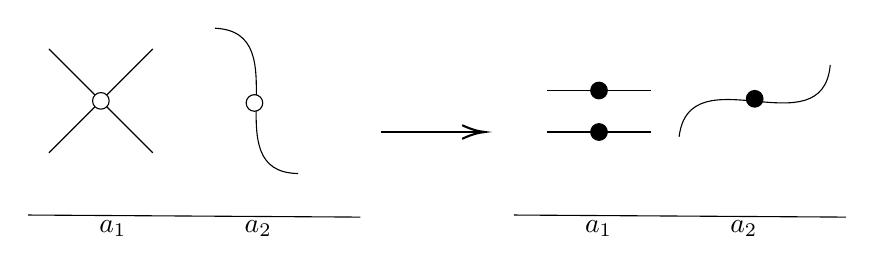
\begin{tikzpicture}[x=0.75pt,y=0.75pt,yscale=-1,xscale=1]
%uncomment if require: \path (0,300); %set diagram left start at 0, and has height of 300

%Straight Lines [id:da7921307799624285] 
\draw    (40,210) -- (200,211) ;
%Straight Lines [id:da09521441359367666] 
\draw    (50,130) -- (100,180) ;
%Straight Lines [id:da020063762282957143] 
\draw    (50,180) -- (100,130) ;
%Curve Lines [id:da731350037149769] 
\draw    (130,120) .. controls (170.8,121.8) and (128.8,189.4) .. (170,190) ;
%Shape: Circle [id:dp13687908959812067] 
\draw  [fill={rgb, 255:red, 255; green, 255; blue, 255 }  ,fill opacity=1 ] (71,155) .. controls (71,152.79) and (72.79,151) .. (75,151) .. controls (77.21,151) and (79,152.79) .. (79,155) .. controls (79,157.21) and (77.21,159) .. (75,159) .. controls (72.79,159) and (71,157.21) .. (71,155) -- cycle ;
%Shape: Circle [id:dp6640632265067969] 
\draw  [fill={rgb, 255:red, 255; green, 255; blue, 255 }  ,fill opacity=1 ] (145,156) .. controls (145,153.79) and (146.79,152) .. (149,152) .. controls (151.21,152) and (153,153.79) .. (153,156) .. controls (153,158.21) and (151.21,160) .. (149,160) .. controls (146.79,160) and (145,158.21) .. (145,156) -- cycle ;
%Straight Lines [id:da6194209106812342] 
\draw    (210,170) -- (258,170) ;
\draw [shift={(260,170)}, rotate = 180] [color={rgb, 255:red, 0; green, 0; blue, 0 }  ][line width=0.75]    (10.93,-3.29) .. controls (6.95,-1.4) and (3.31,-0.3) .. (0,0) .. controls (3.31,0.3) and (6.95,1.4) .. (10.93,3.29)   ;
%Straight Lines [id:da3998897680030452] 
\draw    (274,210) -- (434,211) ;
%Curve Lines [id:da05981114649268304] 
\draw    (353.59,172.3) .. controls (358.47,131.75) and (422.7,178.74) .. (426.41,137.7) ;
%Straight Lines [id:da12513542925991905] 
\draw    (290,150) -- (340,150) ;
%Straight Lines [id:da5201289684803391] 
\draw    (290,170) -- (340,170) ;
%Shape: Circle [id:dp9739499843903215] 
\draw  [fill={rgb, 255:red, 0; green, 0; blue, 0 }  ,fill opacity=1 ] (311,150) .. controls (311,147.79) and (312.79,146) .. (315,146) .. controls (317.21,146) and (319,147.79) .. (319,150) .. controls (319,152.21) and (317.21,154) .. (315,154) .. controls (312.79,154) and (311,152.21) .. (311,150) -- cycle ;
%Shape: Circle [id:dp95739528692497] 
\draw  [fill={rgb, 255:red, 0; green, 0; blue, 0 }  ,fill opacity=1 ] (311,170) .. controls (311,167.79) and (312.79,166) .. (315,166) .. controls (317.21,166) and (319,167.79) .. (319,170) .. controls (319,172.21) and (317.21,174) .. (315,174) .. controls (312.79,174) and (311,172.21) .. (311,170) -- cycle ;
%Shape: Circle [id:dp3851233234387953] 
\draw  [fill={rgb, 255:red, 0; green, 0; blue, 0 }  ,fill opacity=1 ] (386,154) .. controls (386,151.79) and (387.79,150) .. (390,150) .. controls (392.21,150) and (394,151.79) .. (394,154) .. controls (394,156.21) and (392.21,158) .. (390,158) .. controls (387.79,158) and (386,156.21) .. (386,154) -- cycle ;

% Text Node
\draw (73,211.4) node [anchor=north west][inner sep=0.75pt]    {$a_{1}$};
% Text Node
\draw (143,211.4) node [anchor=north west][inner sep=0.75pt]    {$a_{2}$};
% Text Node
\draw (307,211.4) node [anchor=north west][inner sep=0.75pt]    {$a_{1}$};
% Text Node
\draw (377,211.4) node [anchor=north west][inner sep=0.75pt]    {$a_{2}$};
\end{tikzpicture}
\end{center}

Explicitly: Choose a point $a \in S$, and let $\Delta = \Delta_\veps$ be a small disk around $a$ with $\Delta \cap S = \{a\}$. If $a = \infty$, set $\Delta_\veps = \{|z|>1/\veps\} \cup \{\infty\}$. Then,
$$\pi^{-1}(\Delta^*) = U_1 \cup \cdots \cup U_k$$ has finitely many connected components $U_j$, $j=1,\dots,k$. Let $\pi_j:= \pi|_{U_j}: U_j \to \Delta^*$ be a covering map for all $j$. By the theory of covering spaces, there exists positive integers $m_1,\dots,m_k$ and $\varphi_j:U _j \arr[\sim]\Delta^*$ such that the diagram
% https://q.uiver.app/#q=WzAsNCxbMCwwLCJVX2oiXSxbMiwwLCJcXERlbHRhXioiXSxbMCwyLCJcXERlbHRhXioiXSxbMiwyLCJcXERlbHRhXioiXSxbMCwxLCJcXHZhcnBoaV9qIl0sWzAsMiwiXFxwaV9qIiwyXSxbMiwzLCJcXGlkIiwyXSxbMSwzLCJ6IFxcbWFwc3RvIHpee21fan0iXSxbMCwxLCJcXHNpbSIsMl1d
\[\begin{tikzcd}[ampersand replacement=\&,cramped]
	{U_j} \&\& {\Delta^*} \\
	\\
	{\Delta^*} \&\& {\Delta^*}
	\arrow["{\varphi_j}", from=1-1, to=1-3]
	\arrow["\sim"', from=1-1, to=1-3]
	\arrow["{\pi_j}"', from=1-1, to=3-1]
	\arrow["{z \mapsto z^{m_j}}", from=1-3, to=3-3]
	\arrow["\id"', from=3-1, to=3-3]
\end{tikzcd}\]
commutes for all $j=1,\dots,k$. If $D \subset \Delta$ is a disk around $0$, then $\pi_j^{-1}(D)$ is connected. Now, add a point $P_{j,a}$ to $Y$ for each $U_j$, and define a neighborhood of $P_{j,a}$ to be $V_{j,a}:= U_j \cup \{P_{j,a}\}$, with a map
$$\tilde{\varphi_j}:V_{j,a}\to \Delta^* \cup \{ a\}, \quad P_{j,a}\maps 0$$
extending $\varphi_j$. Let $X$ be the completed space, and define $p:X \to \P^1$ by setting $p|_Y=\pi$ and $p(P_{j,a})=a$ for all $j,a$. The complex structure on $X$ is determined by the open covering
$$\mc U := \{ V_{j,a}\} \cup \brax{ U \subset Y \setbar \pi|_U \text{ is a homeomorphism onto an open set in } \C}$$
with charts $\varphi_{V_{j,a}}: V_{j,a}\to \Delta$ the map constructed above, and $\varphi_U:U \to \C$ being $\pi|_U$. Since $\pi :Y \to \P^1\setminus S$ is proper, we deduce that $p:X \to \P^1$ is proper, so $X$ is compact.

Let $\w{pr}_2:V \to \C$ be the second projection, where $V=V(P)$. Then, the function $f:= \w{pr}_2|_Y$ is holomorphic. 

\begin{claim}
    $f$ extends to a meromorphic function on $X$.
\end{claim}

\begin{proof}
    Let $a \in S, x \in X$ with $p(x)=a$, and choose local coordinates $z$ at $x$ and $w$ at $a$ so that $p$ becomes $z \mapsto z^m=w$. If $U$ is a neighborhood by $x$, then by definition of $V$ and $f$, we have $$f(z)^n+\frac{a_1(w)}{a_0(w)}f(z)^{n-1}+\cdots + \frac{a_n(w)}{a_0(w)}=0$$
    for $z \neq 0, w=p(z)$. Also, the functions $a_i(w)/a_0(w)$ are clearly meromorphic at $w=0$, so there exists constant $C,N>0$ such that 
    $$\abs{\frac{a_i(w)}{a_0(w)}}\leq \frac{C}{|w|^N}$$
    near $w=0$. Then, by \Cref{lem:rootbound}, 
    $$|f(z)| \leq 2 \max_i \frac{C^{1/i}}{|w|^{N/i}}\leq \frac{C_1}{|z|^k}$$
    for some constants $C_1$ and $k$. Hence, $f$ has a meromorphic extension to all of $X$.
\end{proof}

\begin{prop}
    $Y$ is connected, so $X$ is as well. Therefore, $X$ is a compact Riemann surface which carries a meromorphic function $f:X \to \P^1$. Moreover, if $p:X \to \P^1$ is the extension of $\pi:Y \to \P^1 \setminus S$, then we have $P(p(x),f(x))=0$ on $X$.
\end{prop}

\begin{proof}
    Suppose $Y$ is not connected, and let $Y_1$ be a connected component of $Y$, $Y_1 \neq Y$. Then, $\pi_1:= \pi|_{Y_1}:Y_1 \to \P^1 \setminus S$ is an $r$-sheeted covering map for some $r$ with $1 \leq r < n$. Let $f_1:=f|_{Y_1}$.

    For any $x \in \P^1 \setminus S$, let $e_\nu$ for $\nu=1,\dots,r$ be the $\nu^{\text{th}}$ elementary symmetric function $e_\nu(x):=e_\nu(y_1,\dots,y_r)$, where $y_1,\dots,y_r$ are the values taken by $f_1$ at the $r$ points of $\pi^{-1}_1(x)$. By definition of $f_1$, the $y_j$ are are values of the $2^{\text{nd}}$ projection $\w{pr}_2$ at the points $(x,y) \in Y$, so we have $P(x,y_j)=0$ for $1 \leq j \leq r$.

    \begin{claim}
        The $e_\nu(x)$ extend to meromorphic functions on $\P^1$.
    \end{claim}

    \begin{proof}
        Indeed, since the $y_j$ are values of the function $f_1$, which is meromorphic on $Y_1$, in a neighborhood of any $a \in S$, since $\pi_1^{-1}(x) = \{P_1,\dots,P_r\}$, we have an estimate
        $$|e_\nu(x)| = \abs{\sum_{i_1<\cdots < i_\nu} f_1(P_{i_1})\cdots f_1(P_{i_\nu})} \leq C \norm{z}^{-\ell}.$$
        Here, $z=(z_1,\dots,z_r)$, where $z_i$ is a coordinate function near $P_i$ for $i=1,\dots,r$. Thus,
        $$|e_\nu(x)| \leq C_1 |x-a|^{-\ell'}$$
        (or $C_1|x|^{-\ell}$ if $a = \infty$), proving that the $e_\nu$ are meromorphic on $\P^1$.
    \end{proof}
    This claim implies that $e_1(x),\dots,e_r(x)$ are rational functions of $x$. Let
    $$Q(x,y) := y^r-e_1(x)y^{r-1}+\cdots + (-1)^re_r(x).$$
    Then, if $x \in \P^1 \setminus S$, the roots $y_1,\dots,y_r$ of $Q(x,y)$ are also roots of $P(x,y)$. Hence, $Q$ divides $P$ in $\C(x)[y]$, and since $\deg_y Q\geq 1$, Gauss's Lemma implies that $P$ is not irreducible in $\C[x][y]$, a contradiction.
\end{proof}

\begin{defn}
    In algebraic geometry, $X$ is called the \textbf{normalization} of the algebraic curve $V=V(P)$
\end{defn}


\section{\texorpdfstring{The Equation $\partial u/\partial \bar z=f$}{The Equation du/dzbar = f}}

Let $R$ be a closed rectangle in $\C$, and $f \in C^{\infty}(R)$ (that is, $f$ is $C^\infty$ in an open neighborhood of $R$).

\begin{prop}[][label=prop:sortastokes]
    $$\iint_R\partder{f}{\bar z}dz\land d\bar z = -\int_{\partial R}f dz,$$
    where $dz \land d \bar z = (dx+idy)\land (dx - idy)=-2i\,dx \land dy$
\end{prop}

\begin{proof}
    Suppose $R=[a,b]\times [c,d]$, and parametrize the four sides of $\partial R$ by $\gamma_1,\gamma_2,\gamma_3,\gamma_4$. Then,
    \begin{align*}
        \iint_R \partder{f}{\bar z}dz \land d \bar z &=-i \int_{c}^d\int_a^b\paren{\partder{f}{x}+i\partder{f}{y}}dxdy
        \\ &= -i\int_c^d \braks{f(b,y)-f(a,y)}dy
        \\ &=-\int_{\gamma_2}fdz -\int_{\gamma_4}fdz.
    \end{align*}
    The rest is an exercise.
\end{proof}

Next, let $R'$ and $R$ be closed rectangles with $R' \subset \Int(R)$. Choose $f$ in some closed annulus $C^\infty (R\setminus \Int(R'))$.
\begin{claim}
    We claim
    $$\iint_{R\setminus \Int(R')}\partder{f}{\bar z}dz \land d\bar z = -\int_{\partial R}fdz + \int_{\partial R'}fdz.$$
\end{claim}
\begin{proof}
    We have $f \in C^\infty (U)$ for some open set $U \supset R\setminus \Int (R')$. Let $\alpha \in C^\infty _0(U)$ with $\alpha \equiv 1$ in a neighborhood of $R\setminus \Int(R')$ (the $0$ in the subscript means compactly supported). Consider
    $$g(z) :=\case{\alpha(z)f(z) & z \in U \\ 0 & z \not \in U.}$$
    Then, $g \in C^\infty (\C)$. Applying \Cref{prop:sortastokes} to $g$ on $R$ and $R'$, we obtain
    $$\iint_R \partder{g}{\bar z}dz \land d\bar z = -\int_{\partial R}f, \quad \iint_{R'}\partder{g}{\bar z}dz \land d\bar z=-\int_{\partial R'}f,$$
    and subtracting gives the claim.
\end{proof}

\begin{thm}[][label=thm:fisdoubleint]
    Let $f \in C_0^\infty (\C)$. Then, for any $\omega \in \C$,
    \begin{align} \label{eq:fisdoubleint}
        f(w) = \frac{1}{2\pi i }\iint_\C \partder{f}{\bar z}(z)\cdot  \frac{1}{z-w}dz \land d \bar z
    \end{align}
\end{thm}

\begin{proof}
    Observe that the function $z \mapsto \frac{1}{z}$ for $0 < |z| \leq 1$ lies in $L^1(\bar D(0,1))$, i.e.
    $$\iint_{|z|\leq 1}\frac{1}{|z|}dxdy < \infty.$$
    (Indeed, passing to polar coordinates shows that the integral equals $2\pi$). We now change variables in \eqref{eq:fisdoubleint} and consider
    $$I:= \iint_\C \partder{f}{\bar z}(z+w)\frac{1}{z}dz \land d \bar z.$$
    We claim $I = 2\pi i f(w)$.

    Indeed, fix $w$, and choose a closed rectangle $R$ such that $\supp(z \mapsto f(z+w)) \subset \Int (R)$ and $0 \in R$. Let $R_\veps$ be a small square centered at $0$ with side length $\veps$, and $R_\veps \subset R$. Using Lebesgue's dominated convergence theorem, we have
    \begin{align*}
        \iint_\C \partder{f}{\bar z}(z+w) \frac{dz \land d \bar z}{z}&=\iint_\C \partder{}{\bar z} \paren{\frac{f(z+w)}{z}}dz \land d \bar z
        \\ &= \lim_{\veps \to 0}\iint_{R \setminus \Int (R_\veps)}\partder{}{\bar z}\paren{\frac{f(z+w)}{z}}dz \land d\bar z
        \\ &= \lim_{\veps \to 0}\int_{\partial R_\veps}\frac{f(z+w)}{z}dz
        \\ &= 2\pi if(w) + \lim_{\veps \to 0}\int_{\partial R_\veps}\frac{f(z+w)-f(w)}{z}dz.
    \end{align*}
    Then, since $f \in C_0^\infty (\C)$, there exists $M>0$ such that $|f(z+w)-f(w)| \leq M|z|$ for $|z|$ small, hence
    $$\abs{\int_{\partial R_\veps}\frac{f(z+w)-f(w)}{z}dz}\leq M\cdot 4\veps \to 0,$$
    proving the claim.
\end{proof}

\begin{thm}[][label=thm:fispartder]
    Let $f \in C_0^\infty (\C)$, and define 
    $$u(w) := \frac{1}{2\pi i }\iint_\C \frac{f(z)}{z-w}dz \land d \bar z.$$
    Then, $u \in C^\infty (\C)$, and $\partder{u}{\bar z}=f$ on $\C$.
\end{thm}

\begin{proof}
    We change variables in the integral so that
    $$u(w) = \frac{1}{2\pi i } \iint _\C \frac{f(z+w)}{z}dz\land d \bar z.$$
    We claim $$\partder{u}{x}(w) =\frac{1}{2\pi i }\iint _\C \frac{\partder{f}{x}(z+w)}{z}dz \land d \bar z.$$
    Indeed, for $h \in \R$,
    $$\frac{u(w+h)-u(w)}{h}=\frac{1}{2\pi i}\iint_\C \frac{f(z+w+h)-f(z+w)}{h}\cdot \frac{1}{z} dz \land d \bar z.$$
    Since $f$ is differentiable, the first factor in the integral is a bounded function of $h$, and $\frac{1}{z}dz \land d\bar z$ is $L^1$ on any compact set, so we obtain the claim by taking the limit as $h \to 0$ (the exchange of limit and integral is justified by the dominated convergence theorem).

    Arguing in the same way shows that $\partder{u}{y}(w) $, and in fact all derivatives of $u$, exist. Hence, $u \in C^\infty (\C)$. Moreover, since $z=x+iy$, and $\partder{}{\bar z}=\frac{1}{2}\paren{\partder{}{x}+i\partder{}{y}}$, we have
    $$\partder{u}{\bar z}(w) = \frac{1}{2 \pi i} \iint_\C \partder{f}{\bar z}(z+w)\frac{1}{z}dz \land d \bar z = f(w)$$
    by \Cref{thm:fisdoubleint}.
\end{proof}

Now, we want to show that $\partder{u}{\bar z}=f$ has a solution for any $f\in C^\infty (\Omega)$, i.e. not necessarily compact supported, and any open $\Omega$. For this, we use Runge's theorem.

\begin{defn}
    Let $\Omega \subset \C$ be open, and $A \subset \Omega$ be any open subset. The \textbf{topological hull} $\hat A_\Omega$ of $A$ in $\Omega$ is the union of $A$ with the connected components of $\Omega \setminus A$ which are relatively compact (closure is compact) in $\Omega$.

    Such a connected component is called a \textbf{hole} of A. Intuitively, one gets $\hat A_\Omega$ by filling the holes of $A$.
\end{defn}

\begin{ex}
We have the following example:


\tikzset{every picture/.style={line width=0.75pt}} %set default line width to 0.75pt        

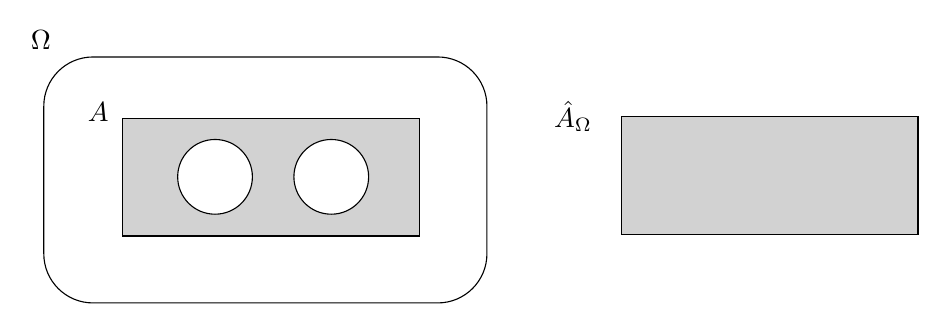
\begin{tikzpicture}[x=0.75pt,y=0.75pt,yscale=-1,xscale=1]
%uncomment if require: \path (0,300); %set diagram left start at 0, and has height of 300

%Rounded Rect [id:dp08608192025104822] 
\draw   (146,90.45) .. controls (146,77.36) and (156.61,66.75) .. (169.7,66.75) -- (335.8,66.75) .. controls (348.89,66.75) and (359.5,77.36) .. (359.5,90.45) -- (359.5,161.55) .. controls (359.5,174.64) and (348.89,185.25) .. (335.8,185.25) -- (169.7,185.25) .. controls (156.61,185.25) and (146,174.64) .. (146,161.55) -- cycle ;
%Shape: Rectangle [id:dp2222508720890346] 
\draw  [fill={rgb, 255:red, 155; green, 155; blue, 155 }  ,fill opacity=0.45 ] (184,96.5) -- (327,96.5) -- (327,153) -- (184,153) -- cycle ;
%Shape: Circle [id:dp29213986219014754] 
\draw  [fill={rgb, 255:red, 255; green, 255; blue, 255 }  ,fill opacity=1 ] (210.5,124.5) .. controls (210.5,114.56) and (218.56,106.5) .. (228.5,106.5) .. controls (238.44,106.5) and (246.5,114.56) .. (246.5,124.5) .. controls (246.5,134.44) and (238.44,142.5) .. (228.5,142.5) .. controls (218.56,142.5) and (210.5,134.44) .. (210.5,124.5) -- cycle ;
%Shape: Circle [id:dp02286357511317405] 
\draw  [fill={rgb, 255:red, 255; green, 255; blue, 255 }  ,fill opacity=1 ] (266.5,124.5) .. controls (266.5,114.56) and (274.56,106.5) .. (284.5,106.5) .. controls (294.44,106.5) and (302.5,114.56) .. (302.5,124.5) .. controls (302.5,134.44) and (294.44,142.5) .. (284.5,142.5) .. controls (274.56,142.5) and (266.5,134.44) .. (266.5,124.5) -- cycle ;
%Shape: Rectangle [id:dp7950584391965025] 
\draw  [fill={rgb, 255:red, 155; green, 155; blue, 155 }  ,fill opacity=0.45 ] (424.2,95.6) -- (567.2,95.6) -- (567.2,152.1) -- (424.2,152.1) -- cycle ;

% Text Node
\draw (138.5,52.9) node [anchor=north west][inner sep=0.75pt]    {$\Omega $};
% Text Node
\draw (166,87.4) node [anchor=north west][inner sep=0.75pt]    {$A$};
% Text Node
\draw (390.6,86.6) node [anchor=north west][inner sep=0.75pt]    {$\hat{A}_{\Omega }$};
\end{tikzpicture}
\end{ex}

\begin{exercise}
    If $A \subset \Omega$, then $\hat{\paren{\hat{A}}}_\Omega=\hat A_\Omega \supset A$. (Don't know what's going on with the TeX here, I'll fix it) 
\end{exercise}

\begin{exercise}
    If $A \subset B \subset \Omega$, then $\hat A_\Omega \subset \hat B_\Omega$.
\end{exercise}

\begin{prop}
    Let $\Omega \subset \C$ be open and $K \subset \Omega$ be compact. Then, $\hat K_\Omega$ is again compact. Moreover, $\C \setminus \hat K_\Omega$ has only finitely many connected components
\end{prop}

\begin{lem}[][label=lem:compact_seq]
    Let $\Omega \subset \C$ be open. Then, there exists a sequence $\{K_n\}_{n \geq 1}$ of compact subsets of $\Omega$ such that 
    \begin{enumerate}[(i)]
        \item $K_n \subset K_{n+1}$,
        \item $\bigcup_{n=1}^\infty K_n = \Omega$,
        \item $K_n = \paren{\hat {K_n}}_\Omega$, i.e. $\Omega \setminus K_n$ has no connected components relatively compact to $\Omega$.
    \end{enumerate}
\end{lem}

\begin{proof}
    We first construct a sequence $\{K_n'\}$ satisfying the first two conditions. 

    If $\Omega = \C$, just use disks $K_n = \bar D(0,n)$. If $\Omega \neq \C$, then $\partial \Omega \neq \emptyset$, so set 
    $$K_n =\brax{x \in \Omega \setbar \w{dist}(x,\partial \Omega) \geq \frac{1}{n}}\cap \bar D(0,n),$$
    and it's easy to show that these satisfy the first two conditions.

    Now, set $K_n := \hat{\paren{K_n'}}_\Omega$ for all $n \geq 1$, and we're done.
\end{proof}

\begin{thm}[Runge's Theorem]
    Let $\Omega \subset \C$ be open and $K \subset \Omega$ be compact. Then, any function $f \in \mc O(\hat K_\Omega)$ can be approximated uniformly on $\hat K_\Omega$, by functions holomorphic on $\Omega$.
\end{thm}

\begin{thm}
    Let $\Omega \subset \C$ be open, and $f \in C^\infty (\Omega)$. Then, there exits $u \in C^\infty (\Omega)$ such that $\partder{u}{\bar z}=f$.
\end{thm}

``The proof is like black magic, and it was by the master of black magic: Grothendieck''.

\begin{proof}[Proof (Grothendieck)]
Let $\{K_n\}_{n \geq1}$ be a sequence of compact subsets of $\Omega$ as in \Cref{lem:compact_seq}. For each $n$, there exists $u_n \in C_0^\infty (\Omega)$ such that $\partder{u_n}{\bar z}=f$ in a neighborhood of $K_n$. Then,
$$\partder{}{\bar z}(u_{n+1}-u_n)=f-f=0$$
in a neighborhood of $K_n$, so $u_{n+1}-u_n \in \mc O(K_n)$. By Runge's Theorem, there exists $h_n \in \mc O(\Omega)$ such that
$$\norm{u_{n+1}-u_n-h_n}_{K_n} < \frac{1}{2^n}$$
for all $n \geq 1$. Now, define $u$ on $K_n$ by
\begin{align} \label{eq:def-of-u}
    u:=u_{n+1}+\sum_{\ell = n}^\infty (u_{\ell+1}-u_{\ell}-h_{\ell})-h_1-h_2-\cdots- h_{n-1},
\end{align}
and observe that the series converges uniformly on $K_n$. Moreover, $u$ is well defined on $\Omega$, since
\begin{align*}
    u&=u_k + \sum_{\ell \geq k}(u_{\ell+1}-u_{\ell}-h_\ell)-\sum_{j<k}h_j
    \\ &= u_k+(u_{k+1}-u_k-h_k)+\sum_{\ell \geq k+1}(u_{\ell+1}-u_{\ell}-h_{\ell})-\sum_{j < k}h_k
    \\ &= u_{k+1}+\sum_{\ell \geq k+1}(u_{\ell+1}-u_\ell -h_\ell) - \sum_{j < k+1}h_j,
\end{align*}
i.e. $u$ is independent of the choice of $n$ for $K_n$. Since the series converges uniformly on $K_n$, we have
$$u-u_{n+1}\in \mc O(K_n)$$
and therefore
$$\partder{u}{\bar z}=\partder{u_{n+1}}{\bar z}=f$$
on $\Int(K_n)$. Since $n$ is arbitrary, and $\bigcup_{n}K_n = \Omega$, we're done.
\end{proof}

\section{Cohomology and the Mittag-Leffler Problem}

\begin{notebox}[The Mittag-Leffler Problem]
   Let $\Omega \subset \C$ be open, $E \subset \Omega$ be discrete, and suppose that for all $a \in E$, we're given a principal part
$$p_a:=\sum_{\nu=1}^\infty \frac{c_\nu}{(z-a)^\nu} \in \mc O(\C \setminus \{a\})$$
where the $c_\nu$ are some given constants.

We ask to find a function $f\in \mc O(\Omega \setminus E)$ such that $f - p_a \in \mc O(a)$ for all $a \in E$.
\end{notebox}

Here is a cohomological approach to the problem: Let $\mc U=\{U_i\}_{i \in I}$ be a covering of $\Omega$ by open sets such that $|U_i \cap E| \leq 1$ for all $i \in I$, and let $f_i$ be any meromorphic function that solves the problem on $U_i$. Note that we can indeed solve the problem on $U_i$, because if $U_i$ contains one point $a \in E$, we can just take $f=p_a$, and otherwise $f$ can be anything holomorphic.

Now, define
$$f_{ij}:=f_i|_{U_i \cap U_j} - f_j|_{U_i \cap U_j} \in \mc O(U_i \cap U_j).$$
Then, on $U_i \cap U_j \cap U_k$, we have $f_{ij}+f_{jk}+f_{ki}=0$. Thus, solving the problem globally on $\Omega$ is equivalent to finding a family of functions $\{g_i \in \mc O(U_i)\}_{i \in I}$ such that $f_{ij}=g_j-g_i$ on $U_i \cap U_j$. for all $i,j \in I$. Indeed, given such a family $\{g_i\}$, we can define $f:= f_i+g_i$ on $U_i$, which is in fact a globally defined function on $\Omega$, because the definition agrees on overlaps. Then, $f$ satisfies the Mittag-Leffler conditions, and conversely a global solution induces such $\{g_i\}$.

In the \v{C}ech cohomology theory, $\{f_{ij}\} : f_{ij}+ f_{jk}+f_{ki}=0$ is a cocylce in $Z^1(\mc U,\mc O)$, and
$$\brax{\{f_{ij}\} \setbar f_{ij}=g_j-g_i \text{ for some } \{g_i\}  }=B^1(\mc U,\mc O)$$
is a coboundary group. The \textbf{first \v{C}ech cohomology group}
$$H^1(\mc U,\mc O):=Z^1(\mc U,\mc O)/B^1 (\mc U,\mc O)$$
is the obstruction to solving the problem in general. The Mittag-Leffler theorem says that this group is zero, for all $\Omega \subset \C$ open, and for all open covers $\mc U$ of $\Omega$.

\section{Sheaves of Abelian Groups}
''Sheaves are friends"
\begin{defn}
    Let $X$ be a topological space. A \textbf{presheaf} $\mc F$ of abelian groups of $X$ is an assignment $U \mapsto \mc F(U)$ of abelian groups $\mc F(U)$ to each open set $U \subset X$, with $F(\emptyset)=0$, and for every pair $V \subset U$ of open sets, there are homomorphisms $r_{U,V}: \mc F(U) \to \mc F(V)$ called \textbf{restriction maps}, satisfying
    \begin{enumerate}[(i)]
        \item $r_{U,U}=\id_{\mc F(U)}$ for all $U \subset X$ open
        \item If $W \subset V \subset U$ are three open sets, then $r_{U,W}=r_{V,W} \circ r_{U,V}$.
    \end{enumerate}
     We usually denote $r_{U,V}(f)$ by $f|_V$, as if $f$ is a function of $U$ and $r_{U,V}(f)$ is its restriction to $V$.

     The presheaf $\mc F$ is called a \textbf{sheaf} if for any $U \subset X$ and open cover $U=\bigcup_{i \in I}U_i$, we have
     \begin{enumerate}[(i)]
        \item If $f,g \in \mc F(U)$ with $r_{U,U_i}(f) = r_{U,U_i}(g)$ for all $i \in I$, then $f=g$.
        \item If we are given, for each $i \in I$, an element $f_i \in \mc F(U_i)$ such that $r_{U_i,U_i \cap U_j}(f_i)=r_{U_j,U_i\cap U_j}(f_j)$ for all $i,j \in I$, then there exists $f \in \mc F(U)$ such that $r_{U,U_i}(f)=f_i$ for all $i \in I$.
     \end{enumerate}
     An element $f \in \mc F(U)$ is called a \textbf{section} of $\mc F$ over $U$.
\end{defn}

\begin{rmk}
    By property (i) of a sheaf, the $f$ in (ii) is unique.
\end{rmk}

\begin{ex}
    Let $X$ be a Riemann surface.
    \begin{enumerate}
        \item \textbf{The sheaf of holomorphic functions $\mc O$}: for any open set $U \subset X$, $\mc O(U)$ is the group of holomorphic functions $U \to \C$
        \item The \textbf{sheaf of $C^\infty$-functions $\mc A$}: for any open set $U \subset X$, \[ \mc A(U) = C^\infty (U):= \{f:U \to C \mid f \text{ is } C^\infty \} \]
        \item \textbf{The presheaf $\mc F$ of constant functions}: $\mc F(U) = \{ f:U \to \C \text{ constant}\}$. Note that $\mc F$ is not a sheaf, as property (ii) fails: if $U$ is disconnected, we can send one component to $0$, another to $1$, and then we can't get a constant function that restricts to $0$ and $1$. However, one gets a sheaf $\C$ by setting $\C(U) := \{ f:U \to \C, f$ is locally constant$\}$.
    \end{enumerate}
\end{ex}

\begin{defn}
    Let $\mc F$ be a presheaf on $X$, and fix $a \in X$. We define an equivalence relation $\sim$ on pairs $(U,f)$, where $U\subset X$ is open with $a \in U$, and $f \in \mc F(U)$ as follows: we say $(U, f) \sim (V,g)$ if there exists $W$ open with $a \in W \subset U \cap V$ such that $f|_W = g|_W$. The equivalence class of a pair $(U,f)$ is called the \textbf{germ} of the section $f$ at $a$, denoted $f_a$. 
    
    The set of all germs of sections at $a$ forms an abelian group $\mc F_a$ called the \textbf{stalk} of $\mc F$ at $a$.
\end{defn}

\begin{notethm*}
    We in fact have
    \[
    F_a := \coprod _{U \ni a} (F(U)/\sim) =: \varinjlim_{U \ni a} \mc F(U) 
    \]
\end{notethm*}
We can associate a sheaf to any presheaf $\mc F$ as follows: Let $|\mc F|=\coprod_{a \in X}\mc F_a$ and $p:|F| \to X$, $f_a \mapsto a$ be the natural projection. Define a topology on $|\mc F|$ as follows: for any $U \subset X$ and $f \in \mc F(U)$, let $N(U,f):=\brax{f_a \setbar a \in U}$, where $f_a$ is the equivalence class inf $\mc F_a$ defined by $(U, f)$. The system of sets $\brax{N(U,f)}_{U \subset X}$ is a basis for a topology on $|\mc F|$ such that $p$ is a local homeomorphism (exercise).

A \textbf{section} of $|\mc F|$ over $U$ is a continuous map $s:U \to |\mc F|$ such that $p \circ s=\id_U$, i.e. $s(a) \in \mc F_a$, for all $a \in U$. Let $|\mc F|(U)$ denote the set of all sections of $|\mc F|$ over $U$.

\begin{exercise}
    $|\mc F|$, together with the natural restriction maps, is a sheaf.
\end{exercise}

\begin{exercise}
    For every $a \in X$, there is a natural isomorphism of stalks
    \[
    \mc F_a \arr[\sim] |\mc F|_a.
    \]
\end{exercise}

\begin{ex}
    If $X$ is a Riemann surface, and $p \in X$, we define the \textbf{skyscraper sheaf} $\C_p$ by
    \[
    \C_p(U) := \case{\C & p \in U, \\ 0 & p \not \in U.}
    \]
    The stalks are
    \[
    (\C_p)_a = \case{0 & a \not \neq p \\ \C & a =p.}
    \]
\end{ex}

\section{\v{C}ech Cohomology of Sheaves}


Let $\mc F$ be a sheaf on the topological space $X$, and $\mc U:= \{U_i\}_{i \in I}$ be an open cover of $X$.
\begin{defn}
    Define \textbf{cochain groups} to be 
    \begin{align*}
        C^0(\mc U,\mc F) &:= \prod_{i \in I}\mc F(U_i) = \brax{ (f_i)_{i \in I} \setbar f_i \in \mc F(U_i), \: \forall i \in I} \\
        C^1 (\mc U,\mc F) &:= \prod_{(i,j)}\mc F(U_i \cap U_j)=\brax{ (f_{ij})_{i \in I} \setbar f_{ij} \in \mc F (U_i \cap U_j), \forall i,j \in I}
    \end{align*}
    Let $Z^1(\mc U,\mc F) \subset C^1(\mc U, \mc F)$ be the subgroup of $\bm 1$\textbf{-cocycles}, consisting of families $(f_{ij})$ for which
    \begin{align} \label{eq:cechcochain}
        f_{ij}+f_{jk}=f_{ik} \quad \text{on } U_i \cap U_j \cap U_k, \: \forall i,j,k \in I
    \end{align}
    Note that \eqref{eq:cechcochain} implies $f_{ii}=0$, and $f_{ij}=-f_{ji}$ for any cocycle $(f_{ij})$.

    Define a \textbf{coboundary map} $\delta: C^0(\mc U,\mc F)\to C^1(\mc U,\mc F)$ by setting $\delta(f_i)_{i\in I}:=(f_{ij})$, where $f_{ij}:= f_j-f_i$ on $U_i \cap U_j$. Moreover, let
    \[ B^1(\mc U,\mc F) := \delta C^0(\mc U,\mc F) \subset Z^1(\mc U,\mc F). \]
    Then, the \textbf{1$\st$ \v{C}ech cohomology group} is
    \[
    H^1(\mc U,\mc F):= Z^1(\mc U,\mc F)/B^1 (\mc U, \mc F).
    \]
    Moreover, the \textbf{0$\th$ cohomology group} is
    \[
    H^0(\mc U,\mc F):= \ker \delta \in C^0(\mc U,\mc F)
    \]
    A $0$-cochain $(f_i)$ belongs to $\ker \delta$ if and only if $f_{i}|_{U_i \cap U_j}=f_j|_{U _i \cap U_j}$ for all $i, j$. Since $\mc F$ is a sheaf, the $f_i$'s come from the restriction of a section $f \in \mc F(X)$. Hence, there exists a natural isomorphism
    \[
    H^0(\mc U,\mc F) \arr[\sim]\mc F(X),
    \]
    so $H^0(\mc U,\mc F)$ is independent of the open cover $\mc U$ of $X$.
\end{defn}

\begin{notethm*}[Goal]
    We aim to study, for any open sets $\Omega \subset \C$, the three groups $H^1(\mc U, \mc A), H^1(\mc U, \mc O)$, and $H^1(\mc U, \mc \C)$ for any open cover $\mc U$ of $\Omega$ by disks.
\end{notethm*}

\subsection{Partitions of Unity}

\begin{defn}
    A \textbf{partition of unity} relative to the open cover $\mc U:=\{U_i\}_{i \in I}$ of $\Omega \subset \C$ is a family $\{\varphi_i\}_{i \in I}$ of $C^\infty$ functions on $\Omega$, such that
    \begin{enumerate}[(i)]
        \item $\varphi_i:\Omega \to \R_{\geq 0}$ has $\supp \varphi_i \subset U_i$,
        \item the family of closed sets $\{\supp \varphi _i\}_{i \in I}$ is \textbf{locally finite}, i.e. for any compact set $K \subset \Omega$, the set $\brax{i \in I \setbar K \cap \supp \varphi_i \neq \emptyset}$ is finite
        \item $\sum_{i \in I}\varphi_i = 1$ on $\Omega$.
    \end{enumerate}
    Partitions of unity always exists for any open cover $\mc U$ of $\Omega$.
\end{defn}

\begin{ex}
    Let $F \subset \Omega$ be a closed subset and $U \subset \Omega$ be an open set containing $F$. Then, there exists $\varphi \in C^\infty (\Omega)$ such that $0 \leq \varphi \leq 1$, $\varphi|_F \equiv 1$, and $\varphi|_{\Omega \setminus U}\equiv 0$.
\end{ex}

\begin{proof}
    Set $U^1 := \Omega \setminus F$, and let $\{\varphi, \varphi'\}$ be a partition of unity relative to the cover $\{U,U'\}$ of $\Omega$. Then, $\varphi'|_F \equiv 0 \implies \varphi|_F \equiv 1$, so $\varphi$ satisfies the required conditions.
\end{proof}

\begin{thm}
    Let $\Omega \subset \C$ be open and $\mc U := \{U_i\}_{i \in I}$ be an open cover of $\Omega$. Then,
    \[
    H^1(\mc U,\mc A)=0
    \]
\end{thm}

\begin{proof}
    Suppose that $(f_{ij})\in Z^1(\mc U, \mc A)$, so $f_{ij}+ f_{jk}=f_{ik}$. We seek a family $(f_i)$ such that $f_{ij}=f_j-f_i$ on $U_i \cap U_j$ for all $i,j$.

    Let $(\varphi _i)_{i \in I}$ be a partition of unity relative to $\mc U$. Observe that the function $\varphi_if_{ij}$ can be defined on the set $U_j$ by setting $\varphi_if_{ij}(z):=0$ for $z \in U_j \setminus U_i$. Now, define
    \[
    f_j := \sum_{i \in I}\varphi_i f_{ij} \in \mc A(U_j).
    \]
    Then, for $j,k \in I$, we have on $U_j \cap U_k$ that
    \begin{align*}
        f_k-f_j = \sum_{i} \varphi_i(f_{ik}-f_{ij}) = \sum_{i}\varphi_i (f_{ji} + f_{ik})=f_{jk}\sum_i \varphi_i = f_{jk}.
    \end{align*}
    Hence, $\delta (f_i) = (f_{ij})$.
\end{proof}

\begin{defn}
A sheaf that admits of a partition of unity is called a \textbf{fine sheaf}. So, $\mc A$ is a fine sheaf.
\end{defn}


\begin{thm}[Mittag-Leffler's Theorem, or the 1$\st$ Cousin Problem]
    Let $\Omega$ be open in $\C$, and $\mc U$ an open cover of $\Omega$. Then,
    \[
    H^1(\mc U,\mc O)=0.
    \]
\end{thm}

\begin{proof}

Begin with a $1$-cocycle $(f_{ij})\in Z^1(\mc U,\mc O)$. Let $\alpha _i \in C^\infty (U_i)$ be such that $\alpha_j - \alpha _i = f_{ij}$ on $U_i \cap U_j$ for all $i,j$. Let $u_i := \partial \alpha _i / \partial \bar z$ on $U_i$. Then, $u_i - u_j=0$ on $U_i \cap U_j$, so there exists $u \in C^\infty (\Omega)$ such that $u|_{U_i}=u_i$ for all $i \in I$.

Now, by \Cref{thm:fisdoubleint}, we know there exists $A \in C^\infty (\Omega)$ such that $\partder{A}{\bar z}=u$ on $\Omega$. Define $(f_i)$ by $f_i := \alpha _i - A$ on $U_i$, for all $i \in I$. Then, on $U_i \cap U_j$, $f_j -f_i = \alpha _j -\alpha _i = f_{ij}$, and $\partder{f_i}{\bar z}=u_i-u=0$ on $U_i$ for all $i \in I$.
\end{proof}

Now, we aim to remove our choice of open cover from the definition of the \v{C}ech cohomology groups. Namely, we want to define $H^1(X, \mc F)$.

\begin{defn}
Let $\mc U:=\{U_i\}_{i \in I}$ and $\mc V:= \{V_i\}_{j \in J}$ be two open covers of $X$. Then, $\mc V$ is said to be a \textbf{refinement} of $\mc U$ if there exists a \textbf{refinement map} $\tau :J \to I$ such that $V_j \subset U_{\tau(j)}$ for all $j \in J$. Such a map $\tau$ induces a map
\[
\tau^* : H^1 (\mc U,\mc F) \to H^1 (\mc V,\mc F)
\]
sending $(f_{ij})\in Z^1(\mc U,\mc F)$ to $(g_{\alpha\beta})_{\alpha,\beta \in J}$, where $g_{\alpha \beta}:= f_{\tau(\alpha) \tau (\beta)}|_{V_\alpha \cap V_\beta}$.
\end{defn}

\begin{notethm*}[Check]
    $\tau^*$ depends only on the covering $\mc U$ and $\mc V$, and not the refinement map $\tau$.
\end{notethm*}

\begin{lem}
    If $\sigma,\tau : J \to I$ are two refinement maps, so $V_\beta \subset U_{\sigma(\beta)} \cap U_{\tau (\beta)}$ for all $\beta \in J$, then the induced maps
    \[
    \sigma^*,\tau^* : H^1(\mc U,\mc F) \to H^1(\mc V, \mc F)
    \]
    are equal. Moreover, if $\mc V$ is a refinement of $\mc U$, the (now natural) morphism
    \[
    H^1(\mc U,\mc F) \to H^1(\mc V ,\mc F)
    \]
    is injective.
\end{lem}

\begin{proof}
    Fix $(f_{ij}) \in Z^1(\mc U, \mc F)$. Then, on $V_{\beta _1}\cap V_{\beta_2}$, we have
    \[
    f_{\tau(\beta_1)\tau(\beta_2)}-f_{\sigma(\beta_1)\sigma(\beta_2)}= g_{\beta_1}-g_{\beta_2},
    \]
    where
    \[
    g_{\beta}=f_{\tau(\beta)\sigma(\beta)}|_{V_\beta}.
    \]
    Hence, we see that
    \[
    \brax{ f_{\tau(\beta _1)\tau(\beta_2)} - f_{\sigma(\beta _1)\sigma(\beta _2)}} \in B^1(\mc V, \mc F).
    \]
    This proves $\sigma^* = \tau^*$. Injectivity is left as an exercise.
\end{proof}

Suppose we have three coverings $\mc U,\mc V, \mc W$, with $\mc W < \mc V < \mc U$, where $<$ means refinement. Write, in general, $\tau_{\mc U,\mc V}$ for the induced map $\tau ^*$. Then,
\[
\tau_{\mc V,\mc W} \circ \tau_{\mc U, \mc V} = \tau_{\mc U, \mc W}.
\]
We can therefore define an equivalence relation $\sigma$ on the disjoint union $\coprod_{\mc U} H^1(\mc U,\mc F)$ over all open coverings by saying $\alpha \in H^1(\mc U,\mc F)$ is equivalent to $\beta \in H^1(\mc V, \mc F)$ if there exists a further refinement $\mc W < \mc U$ and $\mc W < \mc V$ such that
\[
\tau_{\mc U,\mc W}(\alpha)= \tau_{\mc V,\mc W}(\beta).
\]
The set of equivalence classes is in fact a group, and is the direct limit of the $H^1(\mc U,\mc F)$. We write this as
\[
H^1(X, \mc F):= \varinjlim_{\mc U} H^1(\mc U,\mc F)= \coprod_{\mc U}H^{1}(\mc U, \mc F)/\sim.
\]
Then, for any open covering $\mc U$ of $X$, the canonical map $H^1(\mc U,\mc F)\to H^1(X,\mc F)$ is injective. Thus, $H^1(X,\mc F)=0 \iff H^1(\mc U,\mc F)=0$ for all open coverings $\mc U$ of $X$.

There is a useful criterion for when an open cover $\mc U$ of $X$ is sufficient to compute $H^1(X,\mc F)$.

\begin{thm}[Leray's Theorem]
Let $\mc F$ be a sheaf of abelian groups on $X$, and $\mc U:= \{U_i\}_{i \in I}$ be an open cover of $X$ such that $H^{1}(U_i, \mc F)=0$ for all $i \in I$. Then,
\[
H^1(X,\mc F) \cong H^1(\mc U,\mc F).
\]
\end{thm}


\end{document}
